\documentclass[10pt,landscape]{article}
\usepackage[utf8]{inputenc}
\usepackage{multicol}
\usepackage{calc}
\usepackage{ifthen}
\usepackage[portrait]{geometry}
\usepackage{amsmath,amsthm,amsfonts,amssymb}
\usepackage{mathtools}
\usepackage{color,graphicx,overpic}
\usepackage{hyperref}
\usepackage{enumerate}
\usepackage{etoolbox} % Required for \appto.
\usepackage{centernot}
\usepackage{xargs}
\usepackage{ifthen}
\usepackage[shortlabels]{enumitem}
\usepackage{xcolor}
\usepackage{multirow}
\usepackage{dcolumn}
\usepackage{tikz}
\newcolumntype{2}{D{.}{}{2.0}}

\DeclarePairedDelimiter\abs{\lvert}{\rvert}

%%%%%%%%%%%%%%%%%%%%%%%%%%%%%%%%%%%%%%%%%%%%%%%%%%%%%%%%%%%%%%%%%%%%%%%%%%%%%%%%%%%%%%%%%%%%%%

% Define emphasis to be bold face and italic.
\DeclareTextFontCommand{\emph}{\bfseries\em}

% Removes most of whitespace above and below equations.
\newcommand{\zerodisplayskips}{%
  \setlength{\abovedisplayskip}{-5pt}% Default: 12pt plus 3pt minus 9pt
  \setlength{\belowdisplayskip}{3pt}% Default: 0pt plus 3pt
  \setlength{\abovedisplayshortskip}{-5pt}% Default: 12pt plus 3pt minus 9pt
  \setlength{\belowdisplayshortskip}{3pt}% Default: 7pt plus 3pt minus 4pt
}
\appto{\normalsize}{\zerodisplayskips}
\appto{\small}{\zerodisplayskips}
\appto{\footnotesize}{\zerodisplayskips}

%%%%%%%%%%%%%%%%%%%%%%%%%%%%%%%%%%%%%%%%%%%%%%%%%%%%%%%%%%%%%%%%%%%%%%%%%%%%%%%%%%%%%%%%%%%%%%%
% Theorem Environment Setup %
%%%%%%%%%%%%%%%%%%%%%%%%%%%%%%%%%%%%%%%%%%%%%%%%%%%%%%%%%%%%%%%%%%%%%%%%%%%%%%%%%%%%%%%%%%%%%%%
\usepackage{amsthm}

% New environments for definitions and theorems. These will let us put in the
% exact reference to the definition/theorems in the notes, e.g.
%
% \begin{definition}{5.1.1}
%     ...
% \end{definition}
%
% to create a definition with title "Definition 5.1.1", referencing the
% definition with the same number in the notes.
\newenvironment{definition}[1] {
    \par\addvspace{\topsep}
    \noindent\textbf{Definition #1}.
    \ignorespaces
}

\newenvironmentx{theorem}[2][\empty] {

    \newcommand{\Title}{Theorem}

    \ifthenelse{ \equal{#2}{\empty} }{
        % Only one argument supplied, don't need parantheses.
        \par\addvspace{\topsep}
        \noindent\textbf{\Title\  #1}.
        \ignorespaces
    }{
        % Two arguments supplied, show in parantheses.
        \par\addvspace{\topsep}
        \noindent\textbf{\Title\  #1} (#2).
        \ignorespaces
    }
}

\newenvironmentx{lemma}[2][\empty] {

    \newcommand{\Title}{Lemma}

    \ifthenelse{ \equal{#2}{\empty} }{
        % Only one argument supplied, don't need parantheses.
        \par\addvspace{\topsep}
        \noindent\textbf{\Title\  #1}.
        \ignorespaces
    }{
        % Two arguments supplied, show in parantheses.
        \par\addvspace{\topsep}
        \noindent\textbf{\Title\  #1} (#2).
        \ignorespaces
    }
}

\newenvironmentx{proposition}[2][\empty] {

    \newcommand{\Title}{Proposition}

    \ifthenelse{ \equal{#2}{\empty} }{
        % Only one argument supplied, don't need parantheses.
        \par\addvspace{\topsep}
        \noindent\textbf{\Title\  #1}.
        \ignorespaces
    }{
        % Two arguments supplied, show in parantheses.
        \par\addvspace{\topsep}
        \noindent\textbf{\Title\  #1} (#2).
        \ignorespaces
    }
}

\newenvironmentx{corollary}[2][\empty] {

    \newcommand{\Title}{Corollary}

    \ifthenelse{ \equal{#2}{\empty} }{
        % Only one argument supplied, don't need parantheses.
        \par\addvspace{\topsep}
        \noindent\textbf{\Title\  #1}.
        \ignorespaces
    }{
        % Two arguments supplied, show in parantheses.
        \par\addvspace{\topsep}
        \noindent\textbf{\Title\  #1} (#2).
        \ignorespaces
    }
}

\newenvironmentx{remark}[2][\empty] {

    \newcommand{\Title}{Remark}

    \ifthenelse{ \equal{#2}{\empty} }{
        % Only one argument supplied, don't need parantheses.
        \par\addvspace{\topsep}
        \noindent\textbf{\Title\  #1}.
        \ignorespaces
    }{
        % Two arguments supplied, show in parantheses.
        \par\addvspace{\topsep}
        \noindent\textbf{\Title\  #1} (#2).
        \ignorespaces
    }
}

\newenvironmentx{example}[2][\empty] {

    \newcommand{\Title}{Example}

    \ifthenelse{ \equal{#2}{\empty} }{
        % Only one argument supplied, don't need parantheses.
        \par\addvspace{\topsep}
        \noindent\textbf{\Title\  #1}.
        \ignorespaces
    }{
        % Two arguments supplied, show in parantheses.
        \par\addvspace{\topsep}
        \noindent\textbf{\Title\  #1} (#2).
        \ignorespaces
    }
}

\newenvironmentx{exercise}[2][\empty] {

    \newcommand{\Title}{Exercise}

    \ifthenelse{ \equal{#2}{\empty} }{
        % Only one argument supplied, don't need parantheses.
        \par\addvspace{\topsep}
        \noindent\textbf{\Title\  #1}.
        \ignorespaces
    }{
        % Two arguments supplied, show in parantheses.
        \par\addvspace{\topsep}
        \noindent\textbf{\Title\  #1} (#2).
        \ignorespaces
    }
}

\newenvironmentx{question}[2][\empty] {

    \newcommand{\Title}{Question}

    \ifthenelse{ \equal{#2}{\empty} }{
        % Only one argument supplied, don't need parantheses.
        \par\addvspace{\topsep}
        \noindent\textbf{\Title\  #1}.
        \ignorespaces
    }{
        % Two arguments supplied, show in parantheses.
        \par\addvspace{\topsep}
        \noindent\textbf{\Title\  #1} (#2).
        \ignorespaces
    }
}

%%%%%%%%%%%%%%%%%%%%%%%%%%%%%%%%%%%%%%%%%%%%%%%%%%%%%%%%%%%%%%%%%%%%%%%%%%%%%%%%%%%%%%%%%%%%%%%
% Commands for Mathematical Typesetting %
%%%%%%%%%%%%%%%%%%%%%%%%%%%%%%%%%%%%%%%%%%%%%%%%%%%%%%%%%%%%%%%%%%%%%%%%%%%%%%%%%%%%%%%%%%%%%%%

% Redefine \leq and \geq to something nicer looking:
\renewcommand{\leq}{\leqslant}
\renewcommand{\geq}{\geqslant}

% Inner Product:
\DeclareRobustCommand{\InnerProduct}[2]{
    \ifmmode
        \left( #1,#2 \right)
    \else
        \GenericError{\space\space\space\space}
        {Attempting to use \InnerProduct outside of math mode}
    \fi
}

% Vector Norm: 
\DeclareRobustCommand{\Norm}[1]{
    \ifmmode
        \left\lVert #1 \right\rVert
    \else
        \GenericError{\space\space\space\space}
        {Attempting to use \Norm outside of math mode}
    \fi
}

% Image of Function:
\DeclareMathOperator{\im}{im}

% Interior of a Curve:
\DeclareMathOperator{\Int}{Int}

% Exterior of a Curve:
\DeclareMathOperator{\Ext}{Ext}

% Proof Hint:
\newcommand{\Hint}{\textit{Hint: }}

% Real numbers:
\newcommand{\R}{\mathbb{R}}

% Rational numbers:
\newcommand{\Q}{\mathbb{Q}}

% Natural numbers:
\newcommand{\N}{\mathbb{N}}

% Integers:
\newcommand{\Z}{\mathbb{Z}}

% Distance:
\newcommand{\di}[2]{d\left(#1, #2\right)}

% Solution command:
\newcommand{\soln}{\textbf{Solution: }}

% Put a number or letter in parenthesis, bold
\newcommand{\bpar}[1]{\textbf{(#1)}}

% Domain shorthand:
\newcommand{\dom}{\text{dom}}

%%%%%%%%%%%%%%%%%%%%%%%%%%%%%%%%%%%%%%%%%%%%%%%%%%%%%%%%%%%%%%%%%%%%%%%%%%%%%%%%%%%%%%%%%%%%%%%
% PAGE SETUP %
%%%%%%%%%%%%%%%%%%%%%%%%%%%%%%%%%%%%%%%%%%%%%%%%%%%%%%%%%%%%%%%%%%%%%%%%%%%%%%%%%%%%%%%%%%%%%%%

% This sets page margins to .5 inch if using letter paper, and to 1cm
% if using A4 paper. (This probably isn't strictly necessary.)
% If using another size paper, use default 1cm margins.
\ifthenelse{\lengthtest { \paperwidth = 11in}}
    { \geometry{top=.5in,left=.5in,right=.5in,bottom=.5in} }
    {\ifthenelse{ \lengthtest{ \paperwidth = 297mm}}
        {\geometdry{top=1cm,left=1cm,right=1cm,bottom=1cm} }
        {\geometry{top=1cm,left=1cm,right=1cm,bottom=1cm} }
    }

% Turn off header and footer
\pagestyle{empty}

% Redefine section commands to use less space
\makeatletter
\renewcommand{\section}{\@startsection{section}{1}{0mm}%
                                {-1ex plus -.5ex minus -.2ex}%
                                {0.5ex plus .2ex}%x
                                {\normalfont\large\bfseries}}
\renewcommand{\subsection}{\@startsection{subsection}{2}{0mm}%
                                {-1explus -.5ex minus -.2ex}%
                                {0.5ex plus .2ex}%
                                {\normalfont\normalsize\bfseries}}
\renewcommand{\subsubsection}{\@startsection{subsubsection}{3}{0mm}%
                                {-1ex plus -.5ex minus -.2ex}%
                                {1ex plus .2ex}%
                                {\normalfont\small\bfseries}}
\makeatother

% Define BibTeX command
\def\BibTeX{{\rm B\kern-.05em{\sc i\kern-.025em b}\kern-.08em
    T\kern-.1667em\lower.7ex\hbox{E}\kern-.125emX}}

% Don't print section numbers
\setcounter{secnumdepth}{0}


\setlength{\parindent}{0pt}
\setlength{\parskip}{0pt plus 0.5ex}

\setlist[itemize]{leftmargin=0.5cm}
\setlist[enumerate]{leftmargin=0.5cm}

%My Environments
%\newtheorem{example}[section]{Example}
% -----------------------------------------------------------------------

%%%%%%%%%%%%%%%%
% FIGURES %
%%%%%%%%%%%%%%%%
\usepackage{lipsum}
\newenvironment{Figure}
  {\par\medskip\noindent\minipage{\linewidth}}
  {\endminipage\par\medskip}

%%%%%%%%%%%%%%%%%%%%%%%%%%%%%%%%%%%%%%%%%%%%%%%%%%%%%%%%%%%%%%%%%%%%%%%%%%%%%%%%%%%%%%%%%%%%%%%
% SECTION AND SUBSECTION TITLES %
%%%%%%%%%%%%%%%%%%%%%%%%%%%%%%%%%%%%%%%%%%%%%%%%%%%%%%%%%%%%%%%%%%%%%%%%%%%%%%%%%%%%%%%%%%%%%%%
\usepackage[explicit]{titlesec}
\usepackage[normalem]{ulem}
\usepackage{lipsum}

\titleformat{\section}
  {\normalfont\Large}{}{0em}{\uline{\thesection#1}}
\titleformat{name=\section,numberless}
  {\normalfont\Large}{}{0em}{\uline{#1}}

\titleformat{\subsection}
  {\normalfont\normalsize\bfseries}{}{0em}{\uline{\thesection#1}}
\titleformat{name=\subsection,numberless}
  {\normalfont\normalsize\bfseries}{}{0em}{\uline{#1}}

%%%%%%%%%%%%%%%%%%%%%%%%%%%%%%%%%%%%%%%%%%%%%%%%%%%%%%%%%%%%%%%%%%%%%%%%%%%%%%%%%%%%%%%%%%%%%%%
% BEGINNING OF THE DOCUMENT %
%%%%%%%%%%%%%%%%%%%%%%%%%%%%%%%%%%%%%%%%%%%%%%%%%%%%%%%%%%%%%%%%%%%%%%%%%%%%%%%%%%%%%%%%%%%%%%%

\begin{document}
\raggedright
\footnotesize
\begin{multicols}{2}

%%%%%%%%%%%%%%%%%%%%%%%%%%%%%%%%%%%%%%%%%%%%%%%%%%%%%%%%%%%%%%%%%%%%%%%%%%%%%%%%%%%%%%%%%%%%%%%
% MULTICOLS PARAMETERS %
%%%%%%%%%%%%%%%%%%%%%%%%%%%%%%%%%%%%%%%%%%%%%%%%%%%%%%%%%%%%%%%%%%%%%%%%%%%%%%%%%%%%%%%%%%%%%%%
% multicols parameters
% These lengths are set only within the two main columns
%\setlength{\columnseprule}{0.25pt}
\setlength{\premulticols}{1pt}
\setlength{\postmulticols}{1pt}
\setlength{\multicolsep}{1pt}
\setlength{\columnsep}{2pt}
\setlength{\columnseprule}{0.4pt} % For vertical lines separating columns.

%%%%%%%%%%%%%%%%%%%%%%%%%%%%%%%%%%%%%%%%%%%%%%%%%%%%%%%%%%%%%%%%%%%%%%%%%%%%%%%%%%%%%%%%%%%%%%%
% TYPING STARTS HERE %
%%%%%%%%%%%%%%%%%%%%%%%%%%%%%%%%%%%%%%%%%%%%%%%%%%%%%%%%%%%%%%%%%%%%%%%%%%%%%%%%%%%%%%%%%%%%%%%

\begin{center}
    \Large{Combinatorics and Graph Theory Cheatsheet}\\
    \footnotesize{Callum Burgher}\\ 
\end{center}
\scriptsize
\section{1. Definitions}

\begin{itemize}
    \item Simple graph: No loops or multiple edges
    \item General graph: Multiple edges/loops allowed
    \item Vertex set: The set of vertices
    \item Edge set: The set of edges of a graph
    \item Adjacency: (vertex) If there is an edge joining them, (edge) if there is a common vertex
    \item Degree sequence: Sequence of vertex degrees from lowest (left) to highest (right)
    \item \textbf{Handshaking Lemma}: In any graph, the sum of all of the vertex degrees is an even number
    \item Corollary 1.2: In any graph, the number of vertices of odd degree is even
    \item Subgraph: If each vertex/edge belongs to the respective set
    \item Adjacency matrix: $A, B, C, D$ along top and down left, then how many edges between the two
    \item Incidence matrix: Vertices down left, edges across top, 1 if connected, 0 if not
    \item Isomorphism: Two graphs $G_1$ and $G_2$ are \textbf{isomorhpic} if there is a one-to-one correspondence between the vertices of $G_1$ and those of $G_2$, such that the number of edges joining any two vertices of $G_1$ equals the number of edges joining the corresponding vertices of $G_2$
    \item Connected: If the graph cannot be expressed as a union of graphs
    \item Disconnected: If it is not connected
    \item Component: Any disconnected graph $G$ can be expressed as the union of connected graphs, each of which is a component of $G$.
    \item Isolated vertex: A vertex of degree 0
    \item End vertex: A vertex of degree 1
    \item Subgraph: A graph $H$ is a subgraph of $G$ if each of its vertices belong to $V(G)$ and each of its edges belongs to $E(G)$.
    \item Null graphs: A graph whose edge-set is empty is a null graph.
    \item Complete graph: Each pair of distinct vertices are adjacent, $K_n$ with $\frac{n(n-1)}{2}$ edges
    \item Cycle graphs: Each vertex has degree 2, $C_n, n$ vertices
    \item Path graph: Removing an edge from $C_n, P_n, n$ vertices
    \item Wheel: Obtained from $C_{n-1}$ by joining each vertex to a new vertex, $W_n, n$ vertices
    \item Regular graph: Each vertex has same degree
    \item Bipartite: Black to white, in form $G=G(A,B)$
    \item Complete bipartite: A biparite graph where each vertex in $A$ is joined to every vertex in $B$ by exactly one edge, in form $K_{r,s},\ r+s$ vertices, $rs$ edges
    \item Cubic graphs: Regular degree 3, example is the Peterson graph (Pentagon with star in middle)
    \item Platonic graphs: Formed from the vertices and edges of the five regular (Platonic) solids – the tetrahedron, octahedron, cube, icosahedron and dodecahedron \\
    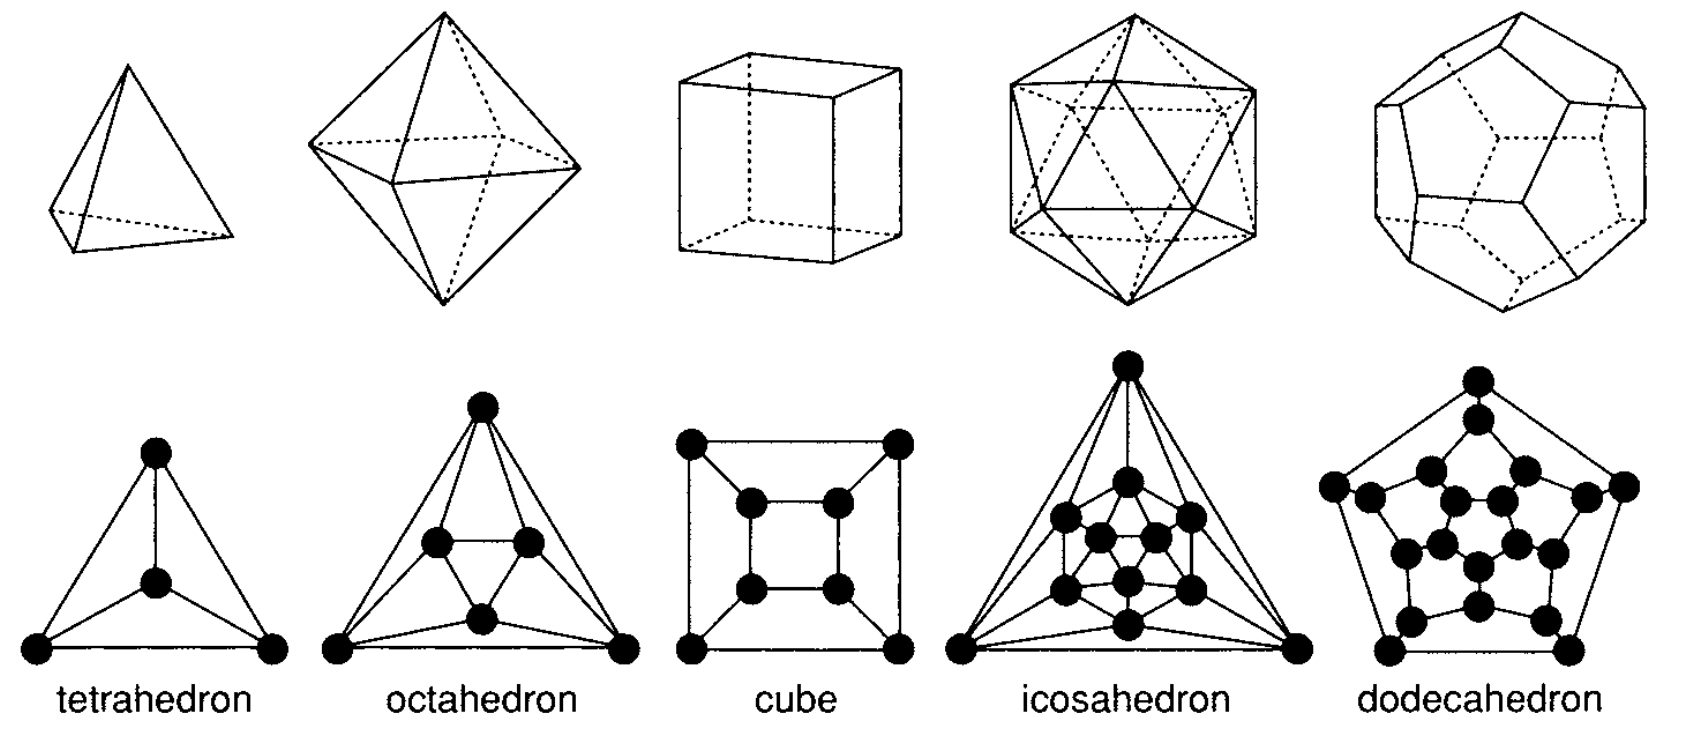
\includegraphics[width = 7cm]{Platonics.png}
    \item Cubes: Among the regular bipartite grpahs. The k-cube $Q_k$ is the graph whose vertices correspond to the sequences ($a_1, a_2,\dots, a_k$) where each $a_i = 0$ or 1. $Q_k$ has $2^k$ vertices and is regular of degree $k$ \\
    \medskip
    \underline{\textbf{Digraphs}}
    \item Digraph: A direted graph
    \item Arc-family: The digraph equivalent of the edge-set
    \item Underlying graph: The graph obtained by removing the arrows from a digraph
    \item Isomorphic: If there is an isomorphism between their underlying graphs
    \item Weakly connected: If it cannot be expressed as the union of two digraphs
    \item Out-degree: $\text{outdeg}(v) \ $\# of arcs $vw$
    \item In-degree: $\text{indeg}(v) \ $\# of arcs $wv$
    \item \textbf{Handshaking Dilemma:} In any digraph the sum of all out-degrees = sum of all in-degrees
    \item Tournament: Any two vertices joined by exactly one arc\\
    \medskip
    \underline{\textbf{Infinite Graphs}}
    \item Infinite graph: Infinite set $V(G)$ of vertices and infinite set $E(G)$ of unordered pairs. If both are countably infinite, then $G$ is a countable graph
    \begin{enumerate}
        \item Locally finite if each vertex has finite degree
        \item Locally countable if each vertex has a countable degree
    \end{enumerate}
    \item \textbf{Thm 1.4}: Every connected locally countable infinite graph is a countable graph
    \item Corollary 1.5: Every locally finite infinite graph is a countable graph
\end{itemize}

\section{2. Paths and Cycles}
\begin{itemize}
    \item Walk: Finite sequence of edges of the form $v_0v_1, v_1v_2, \dots, v_{m-1}v_{m}$
    \item Length: \# edges in a walk
    \item Trail: All distinct edges
    \item Path: A trail with distinct vertices except possibly $v_0=v_m$
    \item Closed: $v_0=v_m$
    \item Cycle: Closed with at least one edge
    \item \textbf{Thm 2.1:} A graph is bipartite $\iff$ every cycle has even length
    \item \textbf{Thm 2.2:} $G$ simple graph on $n$ vertices. If $G$ has $k$ components then the number $m$ of edged of $G$ satisfies $n-k\le m\le\frac{1}{2}(n-k)(n-k+1)$
    \item Corollary 2.3: Any simple graph with $n$ vertices and more than $\frac{1}{2}(n-1)(n-2)$ edges is connected.
    \item Disconnecting set: In a connected graph is a set of edges whose deletion disconnects $G$.
    \item Cutset: A minimal disconnecting set
    \item Bridge: If a cutset only has one edge
    \item Edge-connectivity: If $G$ is connected, then $\lambda(G)$ is the size of the smallest cutset in $G$
    \item K-edge-connected (k-e-c): If $\lambda(G)\ge k$
    \item \textbf{Thm 2.4:} A graph is k-e-c iff any two distinct vertices of $G$ are joined by at least $k$ paths, no two of which have any edges in common
    \item \textbf{Thm 2.5} A graph $G$ with at least $k+1$ vertices is $k$-connected iff any two vertices of $G$ are joined by at least $k$ paths, no two of which have any other vertices in common.
    \item Separating set: In a connected graph G is a set of vertices whose deletion disconnects $G$
    \item Cut vertex: If a separating set contains only one vertex $v$, then $v$ is a cut vertex
    \item Vertex connectivity: The size of the smallest separating set, $\kappa(G)$
    \item We also say $G$ is $k$-connected if $\kappa(G)\ge k$
    \item Strongly connected (\textbf{Digraph}): if for any two vertices of $D$ there is a directed path
    \item Orientable: If each edge of $G$ can be directed so that the resulting digraph $D$ is strongly connected; such a digraph is an \textbf{orientation} of $G$.
    \item \textbf{Thm 2.6:} A connected graph $G$ is orientable iff each edge of $G$ lies in at least 1 cycle
    \item \textbf{Infinite graphs} \begin{enumerate}
        \item One way: $v_0\to v_1\to \cdots$
        \item Two way: $\cdots\to v_{-2}\to v_{-1}\to v_0\to v_1\to v_2\cdots$
    \end{enumerate}
    \item \textbf{Thm 2.7 (König's Lemma):} Let $G$ be a connected locally finite infinite graph. Then, for any vertex, $v$, of $G$, there exists a one way infinite path with initial vertex $v$
\end{itemize}
    \subsection{2.2 Eulerian Graphs}
\begin{itemize}
    \item Eulerian Graph: A connected graph is Eulerian if there exists a closed trail that includes every edge of $G$; such a trail is a Eulerian trail.
    \item A non-Eulerian graph $G$ is semi-Eulerian if there exists a non closed trail that includes every edge of $G$. Below are Eulerian, S-Eulerian and N-Eulerian graphs respectively\\
    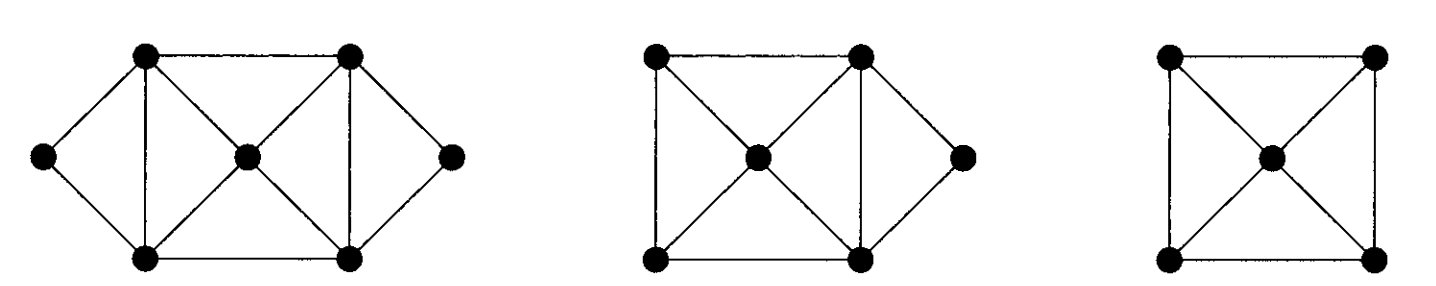
\includegraphics[width = 3 cm]{Eulerian_SE_NE.png}
    \item Lemma 2.8: If $G$ is a graph in which the degree of each vertex is at least 2, then $G$ contains a cycle.
    \item \textbf{Thm 2.9:} A connected graph $G$ is Eulerian iff the degree of each vertex is even
    \item Corollary 2.10: A connected graph is Eulerian iff its set of edges can be split up into edge-disjoint cycles
    \item Corollary 2.11: A connected graph is semi-Eulerian iff it has exactly two vertices of odd degree.
    \item \textbf{Thm 2.12 (Fleury's Algorithm):} Let $G$ be an Eulerian graph. Then the following construction is always possible, and produces an Eulerian trail of $G$. Start at any vertex $u$ an traverse the edges in an arbitrary manner, subject only to the following rules:
    \begin{enumerate}
        \item Erase the edges as they are traversed, and if any isolated vertices result, erase them too 
        \item At each stage, use a bridge only if there is no alternative \textbf{(don't burn your bridges too quick)}
    \end{enumerate}

    \underline{\textbf{Digraphs}}
    \item A connected digraph $D$ is Eulerian if there exists a closed directed trail that includes every arc of $D$.
    \item \textbf{Thm 2.13:} A strongly connected digraph is Eulerian iff, for every vertex $v$ of $D, \ \text{outdeg}(v) = \text{indeg(v)}$ 
    \\
    \underline{\textbf{Infinite graphs}}
    \item \textbf{Thm 2.14:} Let $G$ be a countable connected graph which is Eulerian. Then \begin{enumerate}
        \item $G$ has no vertices of odd degree;
        \item For each finite subgraph $H$ of $G$, the infinite graph $K$ obtained by deleting from $G$ the edges of $H$ has at most two infinite components;
        \item if, in addition, each vertex of $H$ has even degree, then $K$ has exactly one infinite component.
    \end{enumerate}
    \item \textbf{Thm 2.15:} If $G$ is a countable graph, then $G$ is Eulerian iff the above conditions are satisfied
\end{itemize}
    \subsection{2.3 Hamiltonian (Di)graphs}
    \begin{itemize}
        \item Hamiltonian cycle: If there exists a closed trail passing exactly once through each vertex of $G$: such a trail must be a cycle (except $K_1$). Such a cycle is a Hamiltonian cycle
        \item Hamiltonian graph: A graph with a Hamiltonian cycle
        \item Semi-Hamiltonian: A non- Hamiltonian graph is semi-Hamiltonian if there exists a path through every vertex. Below are H, S-H and N-H respectively\\
        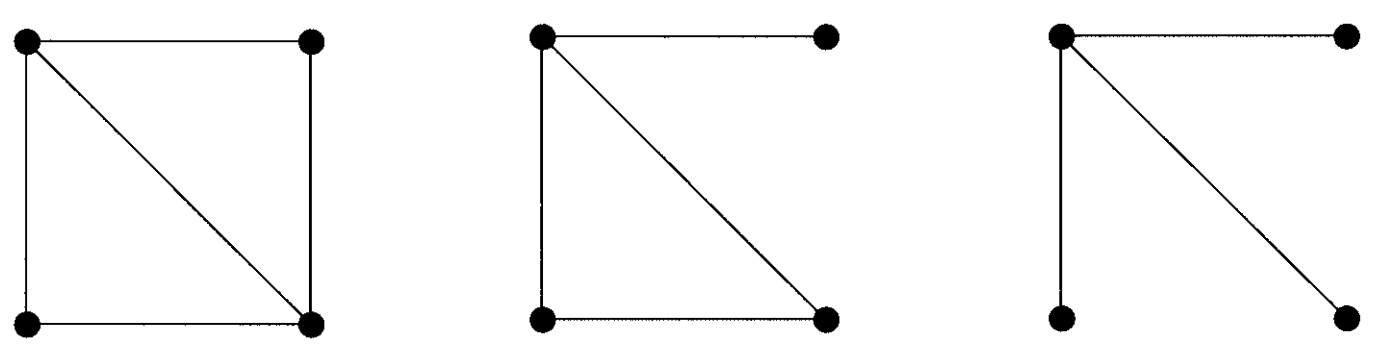
\includegraphics[width = 3 cm]{Hamiltonian_SH_NH.png}
        \item \textbf{Thm 2.16:} If $G$ is a simple graph and if deg$(v) + $deg$(w)\ge n$ for each pair of non-adjacent vertices $v$ and $w$, then $G$ is Hamiltonian.
        \item Corollary 2.17: If $G$ is a simple graph with $n (\ge 3)$ vertices, and if $\text{deg}(v)\ge \frac{n}{2}$ for each vertex $v$, then $G$ is Hamiltonian.
        \item Hamiltonian \textbf{Digraph}: $D$ is Hamiltonian if there is a directed cycle that includes every vertex of $D$.
        \item Semi- HD: A non-Hamiltonian digraph that contains a directed path through every vertex.
        \item \textbf{Thm 2.18:} Let $D$ be a strongly connected digraph with $n$ vertices. If outdeg$(v)\ge \frac{n}{2}$ and indeg$(v)\ge \frac{n}{2}$ for each vertex $v$, then $D$ is Hamiltonian 
        \item \textbf{Thm 2.19:}
        \begin{enumerate}
            \item Every non-Hamiltonian tournament is semi-Hamiltonian (\textbf{Tournament:} Digraph where any two vertices are joined by exactly one arc)
            \item Every strongly connected tournament is Hamiltonian.
        \end{enumerate} 
    \end{itemize}
    \subsection{Applications:}
    \begin{itemize}
        \item Weight: The number assigned to each edge 
        \item Weighted graph: A connected graph in which a non-negative number is assigned to each edge.
    \end{itemize}
    \subsection{The Shortest path problem:} Best shown in an example: See examples section
    \subsection{The Critical path problem} Same as above
    \subsection{The Chinese Postman problem}\begin{itemize}
        \item Eulerian: The shortest path is the Eulerian circuit
        \item Semi-Eulerian:The minimum length of a solution is the total weight added up, plus the shortest path back from one vertex of odd degree to the other
        \item Non-Eulerian: TOO HARD
    \end{itemize} 
    \subsection{The Travelling salesman problem}
    See examples for different questions asked


\section{3. Trees}
\begin{itemize}
    \item Tree: A connected graph that contains no cycles. Trees are simple graph. Any two vertices are connected by exactly one edge
    \item \textbf{Thm 3.1:} Let $T$ be a graph with $n$ vertices. Then the following statements are equivalent:
    \begin{enumerate}
        \item $T$ is a tree
        \item $T$ contains no cycles and has $n-1$ edges
        \item $T$ is connected and has $n-1$ edges
        \item $T$ is connected and each edge is a bridge
        \item Any two vertices of $T$ are connected by exactly one path
        \item $T$ contains no cycles, but the addition of any new edge creates exactly one cycle
        \end{enumerate}
        \item Spanning tree: Given any connected graph $G$, choose a cycle and remove one edge, the resulting graph remains connected, repeating this until there are no cycles and you have one
        \item Cylce rank: The number of edges removed to form a spanning tree, $\gamma(G)=m-n+1 \in \mathbb{Z}^+\cup \{0\}$
        \item Cutset rank: Number of edges in a spanning tree, $\xi(G)=n-1$. Below we have a graph $G$ and one of its spanning trees\\
        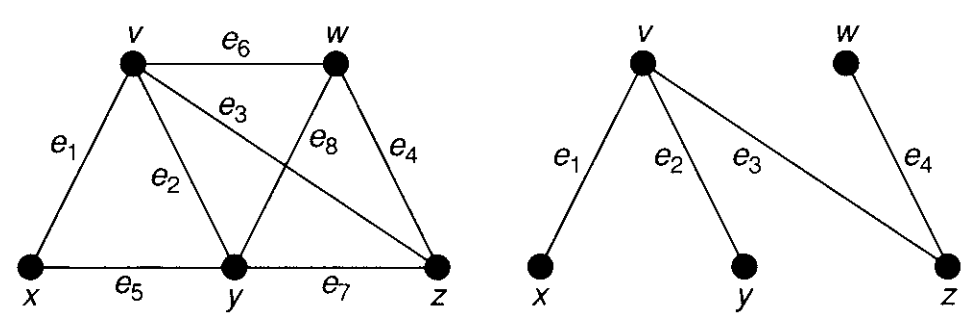
\includegraphics[width = 3cm]{Spanning_Tree.png}
        \item \textbf{Thm 3.2:} If $T$ is any spanning tree of a connected graph $G$, then
        \begin{enumerate}
            \item Each cutset of $G$ has an edge in common with $T$
            \item Each cycle of $G$ has an edge in common with the complement of $T$
        \end{enumerate}
        \subsection{3.2 Counting Trees}
        \item \textbf{Thm 3.3 (Cayley):} There are $n^{n-2}$ distinct labelled trees with $n$ vertices.
        \item Corollary 3.4: The number of spanning trees of $K_n$ is $n^{n-2}$
        \item \textbf{Thm 3.5:} Let $G$ be a connected simple graph with the vertex set $\{v_1, v_2,\dots,v_n\},$ and let $M=(m_{ij})$ be the $n\times n$ matrix in which $m_{ii}=\text{deg}(v_i), m_{ij}= -1$ if $v_i$ and $v_j$ are adjacent, and $m_{ij}=0$ otherwise. Then the number of spanning trees of $G$ is equal to thte cofactor of any element of $M.$ 
        \subsection{3.3 More Applications}

        \subsubsection{The minimum connector problem:}
        \item \textbf{Thm 3.6 (Greedy's Algorithm):} Let $G$ be a connected graph with $n$ vertices. Then the following gives a solution of the minimum connector problem:
        \begin{enumerate}
            \item Let $e_1$ be an edge of $G$ of smallest weight
            \item Define $e_2, e_3,\dots, e_{n-1}$ by choosing at each stage a new edge of smallest possible weight that forms no cycle with the previous edges $e_i$
            The required spanning tree is the subgraph $T$ of $G$ whose edges are $e_1, e_2, \dots, e_{n-1}$
        \end{enumerate}
        \subsubsection{Searching Trees:} The two types are given below: Breadth-first and Depth-first
        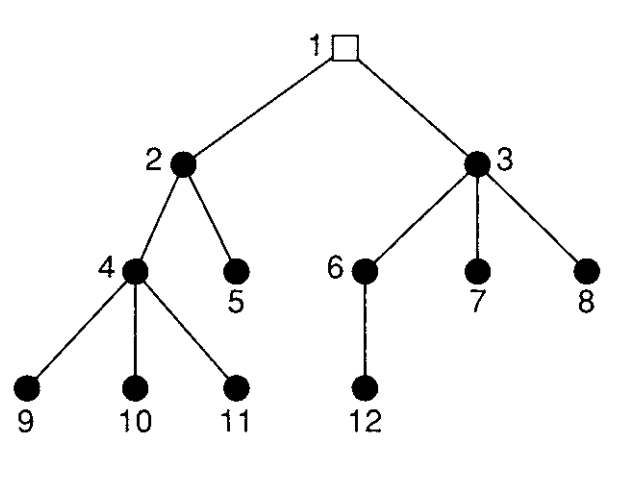
\includegraphics[width=2.5cm, height = 2cm]{BreadthFirst.png}
        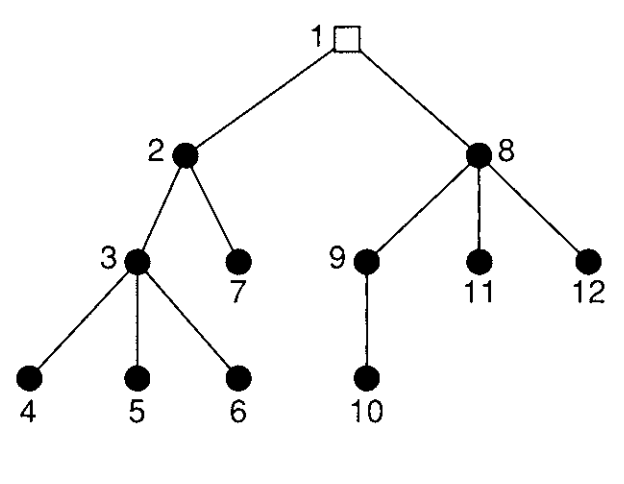
\includegraphics[width=2.5cm]{DepthFirst.png}
        \subsubsection{Bracing Rectangular Frameworks:} 
        \item \textbf{Thm 3.7:} A braced rectangular framework is rigid iff the corresponding bipartite graph is connected. (\textbf{bonus -} If the bipartite graph is a spanning tree, then the bracing is a minimum bracing) \\
        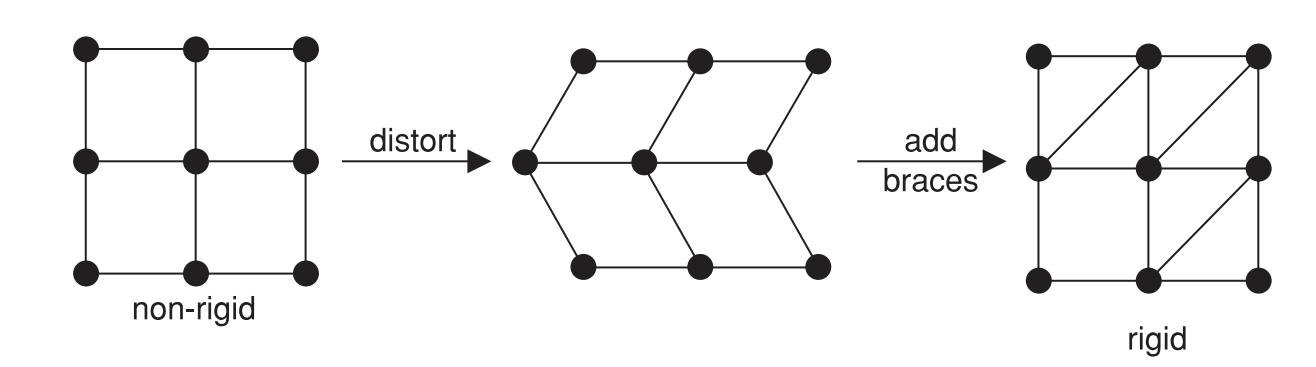
\includegraphics[width = 7cm]{Bracing.png}
        \subsubsection{Electrical Networks:} If we wish to find the current in each wire:
        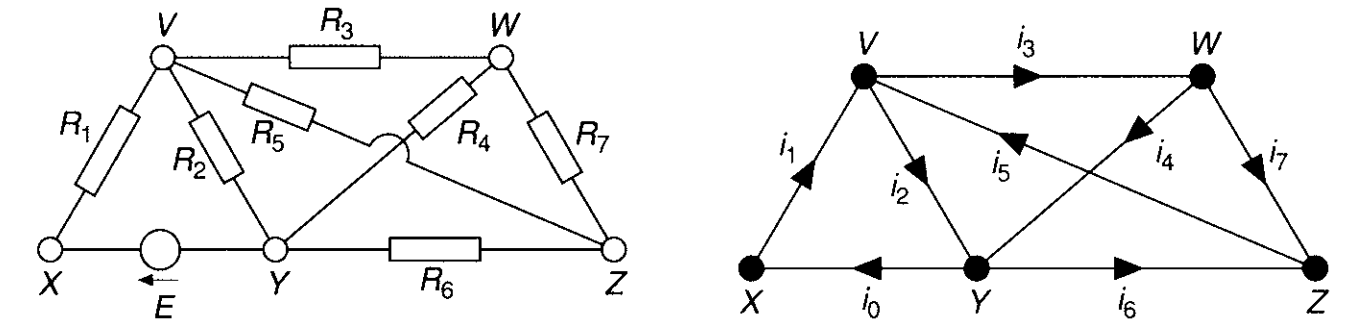
\includegraphics[width = 7cm]{ElectricalNetworks.png}\\
        Assign an arbitrary direction to the current in each wire an apply Kirchoff's Laws:
        \begin{enumerate}
            \item The algebraic sum of the currents at each vertex is 0
            \item The total voltage in each cycle is obtained by adding the products of the currents $i_k$ and resistance $R_k$ in that cycle
        \end{enumerate}
\end{itemize}

\section{4. Planarity}
\subsection{4.1 Planar Graphs}
\begin{itemize}
    \item Planar graph: A graph that can be drawn in the plane without crossings
    \item \textbf{Thm 4.1:} $K_5$ and $K_{3,3}$ are non-planar.
    \item \textbf{Kuratowski's Thm:}
    \begin{enumerate}
        \item Every subgraph of a planar graph is planar
        \item Every graph with a non-planar subgraph is non-planar
    \end{enumerate}
        \item Homeomorphic: Two graphs are said to be homeomorphic if both can be obtained from the same graph by inserting new vertices of degree 2 into its edges
        \item \textbf{Thm 4.2 (Kuratowski):} A graph is planar iff it contains no subgraph homeomorphic to $K_5$ or $K_{3,3}$
        \item Contractible: A graph $H$ is contractible to $K_5$ or $K_{3,3}$ if we can obtain them by successively contracting edges
        \item \textbf{Thm 4.3:} A graph is planar iff it contains no subgraph contractible to $K_5$ or $K_{3,3}$
        \item Every connected graph with 8 or fewer edges is planar
        \item \textbf{Infinite planar graphs (Thm 4.4:)} If $G$ is a countable graph, every finite subgraph of which is planar, then $G$ is planar.

        \subsection{4.2 Euler's Formula}
        If $G$ is planar, then any plane drawing of $G$ divides the set of points of the plane not lying on $G$ into regions, called faces.
        \item \textbf{Thm 4.5 (Euler):} Let $G$ be a plane drawing of a planar graph, and let $n, m$ and $f$ denote respectively the number of vertices, edges and faces of $G$. Then $$n-m+f=2$$
        \item Corollary 4.6: Let $G$ be a polyhedral graph. Then\\ $$n-m+f=2$$
        \item Corollary 4.7: Let $G$ be a plane graph with $n$ vertices, $m$ edges, $f$ faces and $k$ components. Then $$n-m+f = k+1$$
        \item Corollary 4.8: \begin{enumerate}
            \item If $G$ is a simple connected planar graph with $n\ge 3$ vertices and $m$ edges, then $$m\le 3n-6$$
            \item If, in addition, $G$ has no triangles, then \\$$m\le2n-4$$
        \end{enumerate}
        \item \textbf{Thm 4.10:} Every simple planar graph $G$ contains a vertex of degree at most 5
        \item \textbf{Thm 4.11:} Let $G$ be a simple graph with $n\ge3$ vertices and $m$ edges. Then the thickness $t(G)$ of $G$ satisfies the inequalities\\
        $$t(G)\ge \left\lceil\frac{m}{3n-6}\right\rceil \ \ \text{and} \ \ t(G)\ge \left\lfloor \frac{m+3n-7}{3n-6}\right\rfloor$$
    \subsection{4.3 Dual Graphs}
    \item Geometric Dual $(G^*)$: Built from plane drawing of planar graph $G$ as follows:
    \begin{enumerate}
        \item Choose a point $v^*$ in each face $f$ of $G$. These are the vertices of $G^*$
        \item Corresponding to each edge $e$ of $G$ draw a line $e^*$ that crosses \textbf{only} e and joins the vertices $v^*$ in the faces $f$ adjoining $e$, there are the edges of $G^*$ Example below:\\
        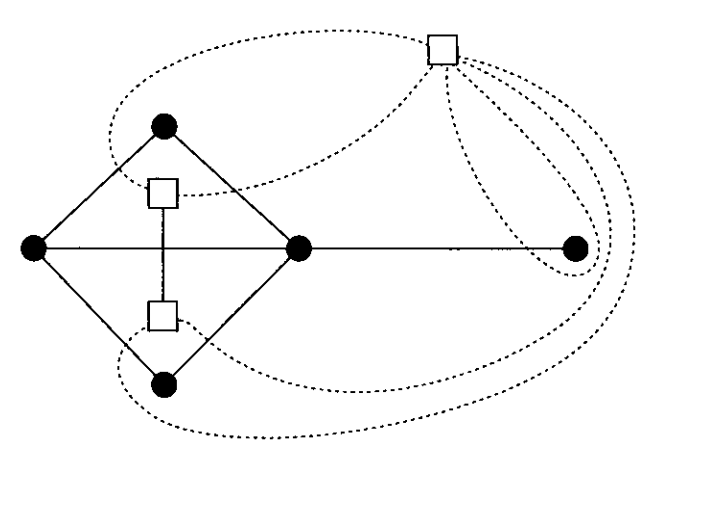
\includegraphics[width = 2cm]{GeomDual.png}
    \end{enumerate}
    \item Lemma 4.12: $G$ connected plane graph, with usual $n$ vertices, $m$ edges and $f$ faces. Its geometric dual $G^*$ has $n^*$ vertices, $m^*$ edges and $f^*$ faces. Then \\
    $$n^*=f,\ m^*=m, \ f^*=n$$
    \item \textbf{Thm 4.13:} If $G$ is a connected plane graph, then $G^**$ is isomorphic to $G$.
    \item \textbf{Thm 4.14:} Let $G$ be a planar graph and let $G^*$ be a geometric dual of $G$. Then a set of edges in $G$ forms a cycle in $G$ iff the corresponding set of edges in $G^*$ forms a cutset in $G^*$
    \item Corollary 4.15: A set of edges of $G$ forms a cutset in $G$ iff the corresponding set of edges of $G^*$ forms a cycle in $G^*$
    \item \textbf{Thm 4.16:} If $G^*$ is an abstract dual of $G.$ Then $G$ is an abstract dual of $G^*$ (\textbf{Abstract dual:} if there is a 1-1 correspondence between the edges of $G$ and those of $G^*,$ with the property from Cor 4.15
    \item \textbf{Thm 4.17:} A graph is planar iff it has an abstract dual.

    \subsection{Graphs on other surfaces}
    \item Genus: A surface is of genus $g$ if it is topologically homeomorphic to a sphere with $g$ handles.
    \item Sphere has genus $0$, Doughnut (torus) has genus $1$
    \item $K_5$ and $K_{3,3}$ are graphs of genus 1
    \item \textbf{Thm 4.18:} The genus of a graph does not exceed the crossing number. (crossing number- the smallest number of crossings, of two edges, that can occur when graph is drawn in the plane)
    \item \textbf{Thm 4.19:} Let $G$ be a connected graph of genus $g$ with $n$ vertices, $m$ edges and $f$ faces. Then \\$$n-m+f=2-2g$$
    \item Corollary 4.20: The genus $g(G)$ of a simple graph $G$ with $n\ge 4$ vertices and $m$ edges satisfies the inequality \\
    $$g(G)\ge \left\lceil \frac{(m-3n}{6}+1\right\rceil$$
    \item \textbf{Thm 4.21:} $g(K_n)=\left\lceil\frac{(n-3)(n-4)}{12}\right\rceil$
    \end{itemize}
    \section{5. Colouring Graphs}
    \subsection{5.1 Colouring Vertices}
    \begin{itemize}
    \item $k$-colourable: If $G$ is a graph with no loops, then $G$ is $k$-colourable if we can assign one of $k$ colours to each vertex so that adjacent vertices have different colours. $W_5$ is 3-colourable as seen below\\
    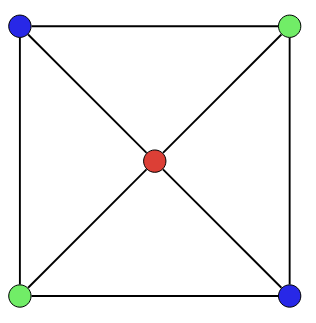
\includegraphics[width = 1.4cm]{3_Colourable_W5.png}
    \item $k$-chromatic: If $G$ is $k$-colourable but not $(k-1)-$colourable, alternatively we say the chromatic number of $G$ is $k$, $\chi(G)=k$.
    \item \textbf{Thm 5.1:} If $G$ is a simple graph with the largest vertex degree $\Delta$, then $G$ is $(\Delta+1)-$colourable.
    \item \textbf{Brooke's Thm (5.2):} If $G$ is a simple connected graph which is not a complete graph, and if the largest vertex-degree is $\Delta\ge 3,$ then $G$ is $\Delta-$colourable
    \item \textbf{Thm 5.3,4,5:} Every simple planar graph is 6, 5, 4-colourable
    \subsection{5.2 Chromatic Polynomials}
    \item Chromatic function: $G$, a simple graph then $P_G(k)$ is the number of ways of colouring the vertices so that no two adjacent vertices have the same colour. $P_G$ is the chromatic polynomial
    \item If $G$ is a simple planar graph, then $P_G(4)>0$
    \item \textbf{Thm 5.6:} Let $G$ be a simple graph, and let $G-e$ and $G\backslash e$ be the graphs obtained by deleting and contracting and edge $e$. Then, \\
    $$P_G(k)=P_{G-e}(k)-P_{G\backslash e}(k)$$
    \item Corollary 5.7: The chromatic function of a simple graph is a polynomial.

    \subsection{5.3 Colouring Maps}
    \item Map: A 3-connected plane graph
    \item $k$-colourable-$(f)$ map: If its faces can be coloured with $k$ colours so that no two faces with a boundary edge in common have the same colour.
    \item \textbf{Thm 5.8:} A map $G$ is 2-colourable-$(f)$ iff $G$ is an Eulerian graph
    \item \textbf{Thm 5.9:} Let $G$ be a plane graph without loops, and let $G^*$ be a geometric dual of $G$. Then $G$ is $k-$colourable-$(v)$ iff $G^*$ is $k-$colourable-$(f)$
    \item Corollary 5.10: The four colour theorem for maps is equivalent to the four colour theorem for planar graphs
    \item \textbf{Thm 5.11:} Let $G$ be a cubic map. Then $G$ is 3-colourable iff each face is bounded by an even number of edges
    \item \textbf{Thm 5.12:} In order to prove the four colour theorem, it is sufficient to prove that every cubic map is 4-colourable-$(f)$
    \subsection{5.4 The Four-Colour Theorem}
    \item Unavoidable sets:\\
    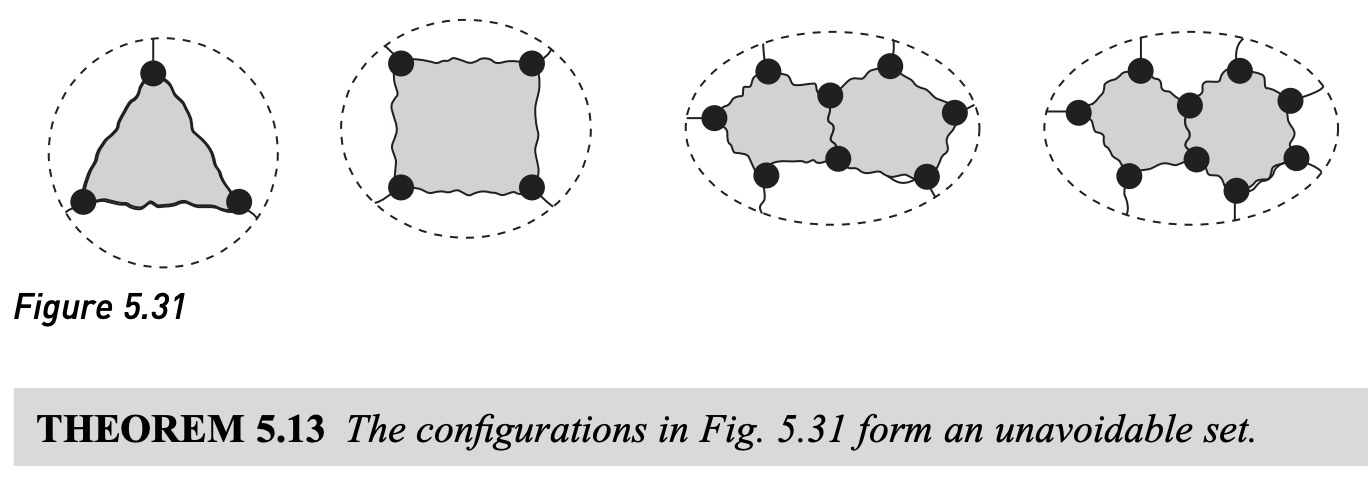
\includegraphics[width = 5.5cm]{UnavoidableSet.png}
    \item Reducible: We say a configuration of faces is reducible if a 4-colouring of all the other faces can be extended (directly or after interchanging colours) to include the configuration
    \item \textbf{Birkhoff Diamond:} Another reducible configuration shown below.\\
    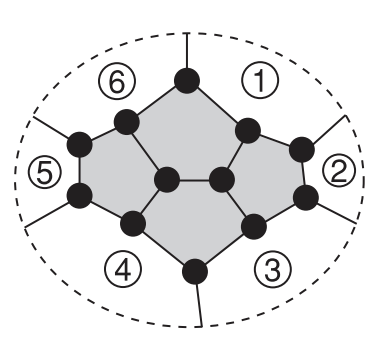
\includegraphics[width = 2cm]{BirkhoffDiamond.png}
    \item \textbf{Thm 5.14:} The Birkhoff diamond is reducible
    \subsection{5.5 Colouring Edges}
    \item $k$-colourable-$(e)$ if its edges can be coloured with $k$ colours so that no two adjacent edges have the same colour 
    \item Chromatic index: If $G$ is $k$-colourable-$(e)$ but not $(k-1)$-colourable-$(e)$, we say that the chromatic index of $G$ is $k$, and we write $\chi'(G)=k$
    \item \textbf{Thm 5.25 (Vizing):} If $G$ is a simple graph with the largest vertex-degree $\Delta$, then\\
    $$\Delta\le\chi'(G)\le\Delta+1$$
    \item \textbf{Thm 5.16:} $\chi'(K_n)=n$ if $n\ge 3$ is odd, and $\chi'(K_n)=n-1$ if $n$ is even
    \item \textbf{Thm 5.17:} The four-colour theorem is equivalent to the statement that $\chi'(G)= 3$ for each cubic map $G$
    \item \textbf{Thm 5.18 (König's):} If $G$ is a bipartite graph with the largest vertex-degree $\Delta$, then $\chi'(G)=\Delta$
    \item Corollary 5.19: $\chi'(K_{r,s})=\text{max}(r,s)$
    \end{itemize}

    \section{6. Matching, Marriage and Menger's Thm}
    \subsection{6.1 Hall's `Marriage' Theorem}
    \begin{itemize}
    \item \textbf{The Marriage Problem:} If there is a finite set of girls, each of whom knows several boys, under what conditions can all the girls marry boys in such a way that each girl marries a boy that she knows.
    \item Complete matching: From $V_1$ to $V_2$ in a bipartite graph $G(V_1, V_2)$ is a one-to-one correspondence between the vertices in $V_1$ and some of the vertices in $V_2$, such that the corresponding vertices are joined. Then the marriage problem can be expressed as: 

    If $G=G(V_1,v_2)$ is a bipartite graph, when does there exist a complete matching from $V_1$ to $V_2$ in $G$
    \item \textbf{Thm 6.1 (Hall):} A necessary and sufficient condition for a solution of the marriage problem is that each set of $k$ girls collectively knows at least $k$ boys, for $1\le k \le m$

    \item Corollary 6.2: Let $G=G(V_1,V_2)$ be a bipartite graph, and for each subset $A$ of $V_1$, let $\varphi(A)$ be the set of vertices of $V_2$ that are adjacent to at least one vertex of $A$. Then a complete matching from $V_1$ to $V_2$ exists iff $|A|\le |\varphi(A)|,$ for each subset $A$ of $V_1$

    \item Transversal: If $E$ is a non-empty finite set, and if $\mathcal{F}=(S_1, S_2,\dots, S_m)$ is a family of non-empty subsets of $E$, then a \textbf{transversal} of $\mathcal{F}$ is a set of $M$ distinct elements of $E$, one chosen from each set $S_i;$ thus, $\{b_4, b_1, b_3, b_2\}$ is a transversal of the family \\ $$\mathcal{F}=(\{b_1, b_4, b_5\}, \{b_1\}, \{b_2, b_3, b_4\}, \{b_2, b_4\})$$
    \item Partial transversal: We call a transversal of a subfamily of $\mathcal{F}$ a \textbf{partial transversal} of $\mathcal{F}$. Note: Any subset of a partial transversal is a partial transversal
    \item \textbf{Thm 6.3:} Let $E$ be a non-empty finite set, and let $\mathcal{F}= (S_1, S_2,\dots, S_m)$ be a family of non-empty subsets of $E$. Then $\mathcal{F}$ has a transversal iff the union of any $k$ of the subsets $S_i$ contains at least $k$ elements, for $1\le k\le m$
    \item If $E$ and $\mathcal{F}$ are as before, then $\mathcal{F}$ has a partial transversal of size $t$ iff the union of any $k$ of the subsets $S_i$ contains at least $k+t-m$ elements

    \subsection{6.2 Menger's Theorem}
    \item Edge-disjoint paths: The maximum number of paths from $v$ to $w$ in a graph $G$, no two of which have an edge in common 
    \item Vertex-disjoint paths: The maximum number of paths from $v$ to $w$, no two of which have a vertex in common
    \item $vw-$disconnecting set: A set $E$ of edges of $E$ such that each path from $v$ to $w$ includes an edge of $E$
    \item $vw-$separating set: A set of $S$ vertices, other than $v$ or $w$ such that each path from $v$ to $w$ passes through a vertex of $S$
    \item \textbf{Thm 6.5:} The maximum number of edge disjoint paths connecting two distinct vertices $v$ and $w$ of a connected graph is equal to the minimum number of edges in a $vw-$disconnedting set 
    \item \textbf{Thm 6.6 (Menger):} The maximum number of vertex-disjoint paths connecting two non-adjacent vertices $v$ and $w$ of a graph is equal to the minimum number of vertices in a $vw-$separating set
    \item Corollary 6.7: A graph $G$ is $k-$edge-connected iff any two distinct vertices of $G$ are connected by at least $k$ edge-disjoint paths
    \item Corollary 6.8: A graph $G$ with at least $k+1$ vertices is $k-$connected iff any two disjoint vertices of $G$ are connected by at least $k$ vertex-disjoint paths
    \item \textbf{Thm 6.9:} The maximum number of arc-disjoint paths from a vertex $V$ to a vertex $w$ in a digraph is equal to the minimum number of arcs in a $vw-$disconnecting set
    \item \textbf{Thm 6.10} Menger's theorem implies Hall's Theorem

    \subsection{6.3 Network Flows}
    \item Network: We define a network $N$ to be a weighted digraph
    \item Capacity: Each arc $a$ is assigned a non-negative real number $c(a)$
    \item The outdeg$(x)$ of a vertex $x$ is the sum of the capacities of the arcs of the form $xz$, indeg$(x)$ is similarly defined
    \item \textbf{Handshaking dilemma for networks:} The sum of the out-degrees of the vertices of a network is equal to the sum of the in-degrees
    \item Source: A vertex with in-deg = 0
    \item Sink: A vertex with an out-deg=0
    \item Flow: A flow in a network is a function $\varphi$ that assigns to each arc $a$ a non-negative real number $\varphi(a),$ called the flow in $a$, in such a way that:\begin{enumerate}
        \item for each arc $a, \varphi(a)\le c(a)$
        \item the out-degree and in-degree of each vertex, other than $v$ or $w$, are equal
    \end{enumerate}
    \item Zero flow: When the flow in every arc is 0, any other flow is a non-zero flow
    \item Saturated: An arc $a$ for which $\varphi(a)=c(a)$, if not then unsaturated
    \item Cut: A set $A$ of arcs such that each path from $v$ to $w$ includes an arc in $A$. A cut in a network is a $vw-$disconnecting set in the corresponding digraph $D$
    \item Capacity of a cut: The sum of the capacities of the arcs in the cut
    \item Minimum cuts: The cuts whose capacity is as small as possible
    \item \textbf{Thm 6.11 (Max-flow Min-cut Theorem):} In any network, the value of any maximum flow is equal to the capacity of any minimum cut
    \item Flow-augmenting paths: Paths that consist entirely of unsaturated arcs $xz$ and $zx$ carrying a non-zero flow
    
\end{itemize}
    

    
\section{7. Examples}

\textbf{Normal 1st Questioners}\\(load of definition testers)

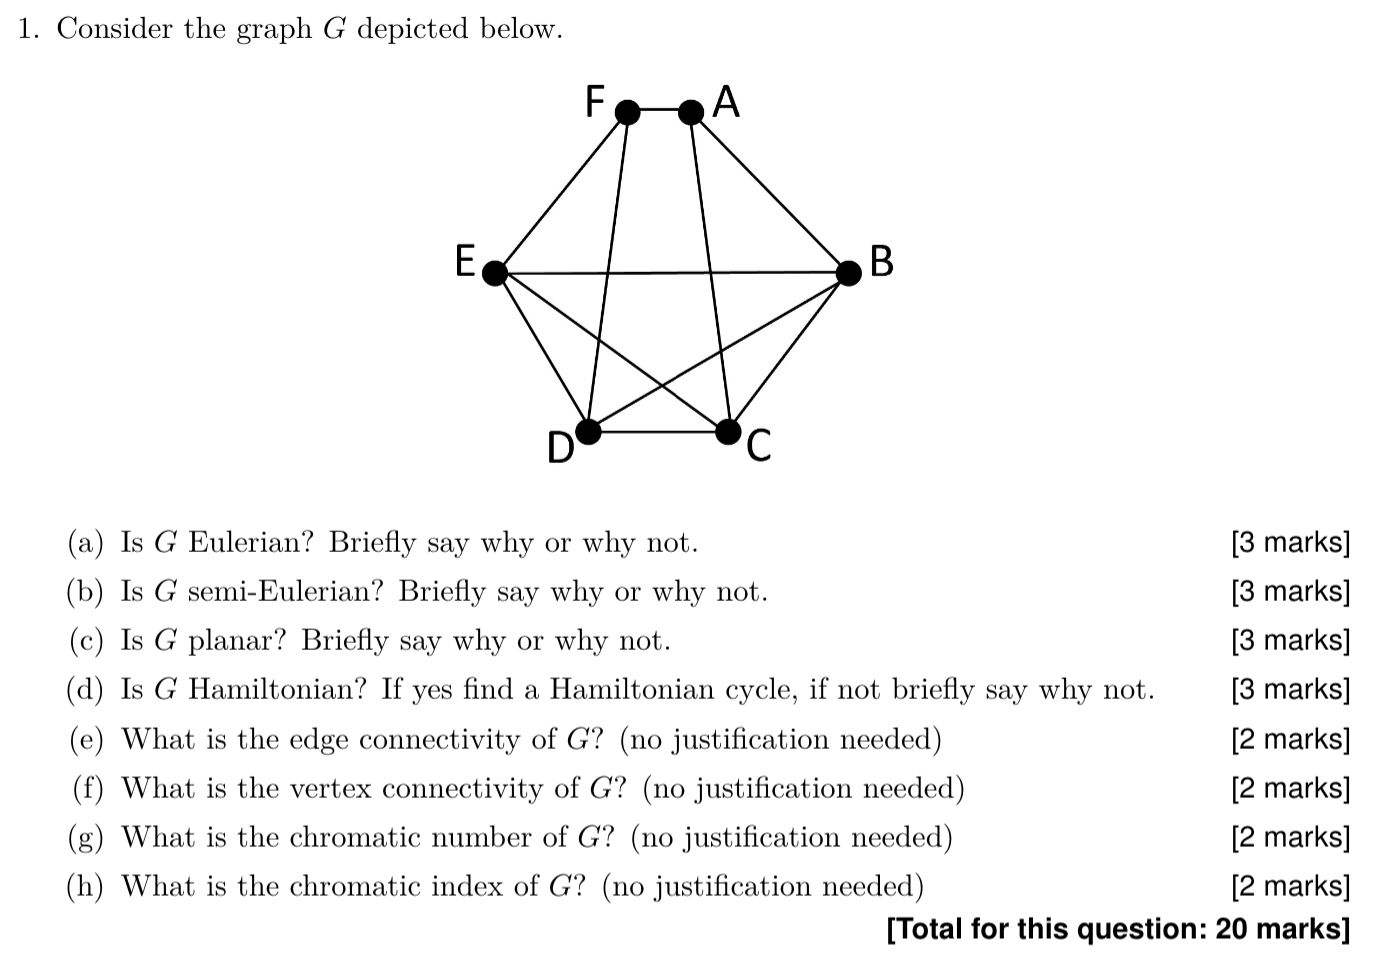
\includegraphics[width = 10 cm]{2023Q1.png}
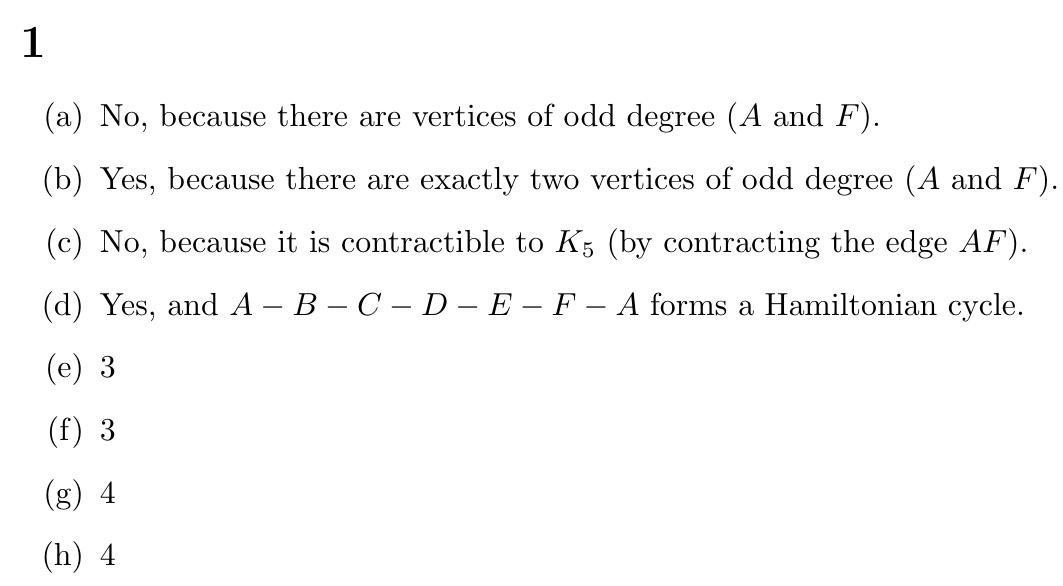
\includegraphics[width = 10 cm]{2023A1.png}

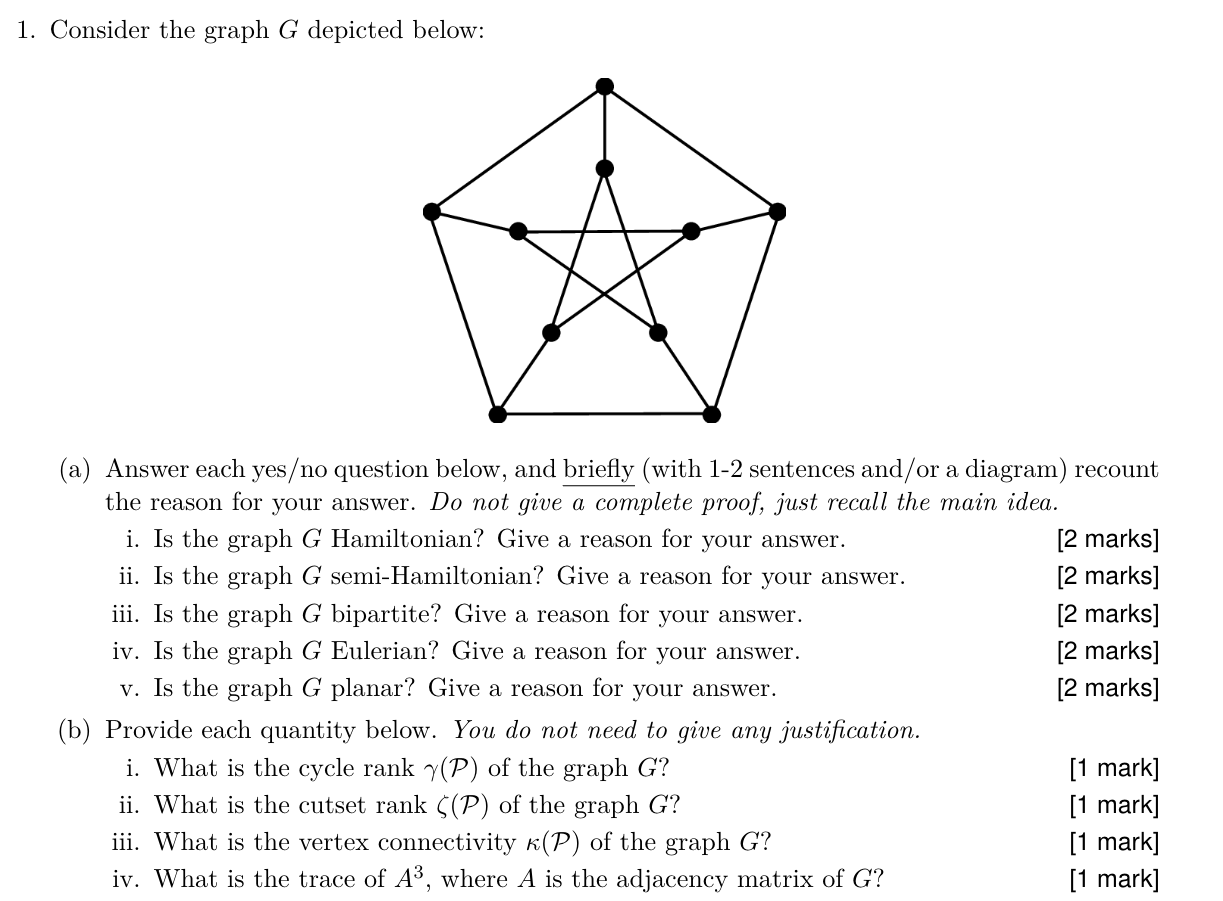
\includegraphics[width = 10 cm]{2022Q1.png}
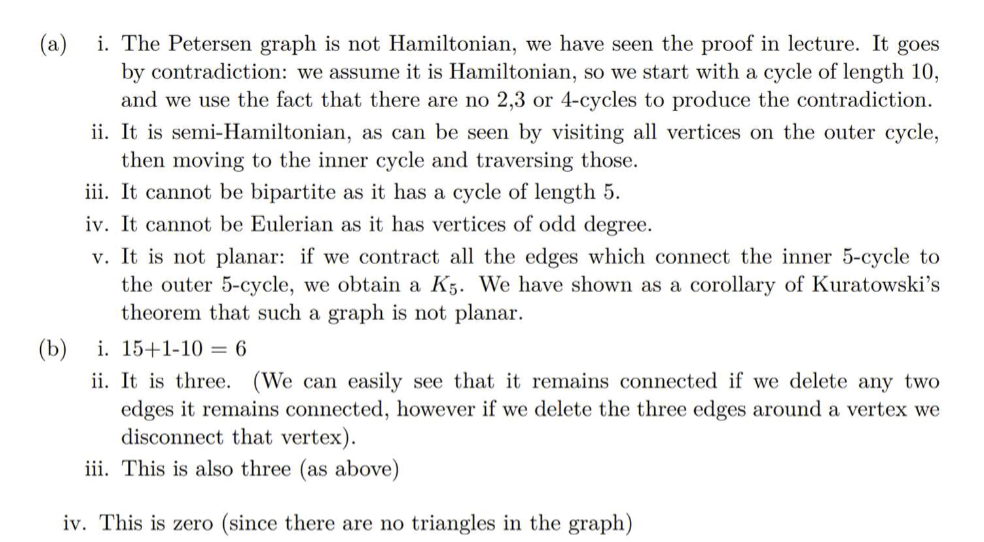
\includegraphics[width = 10 cm]{2022A1.png}
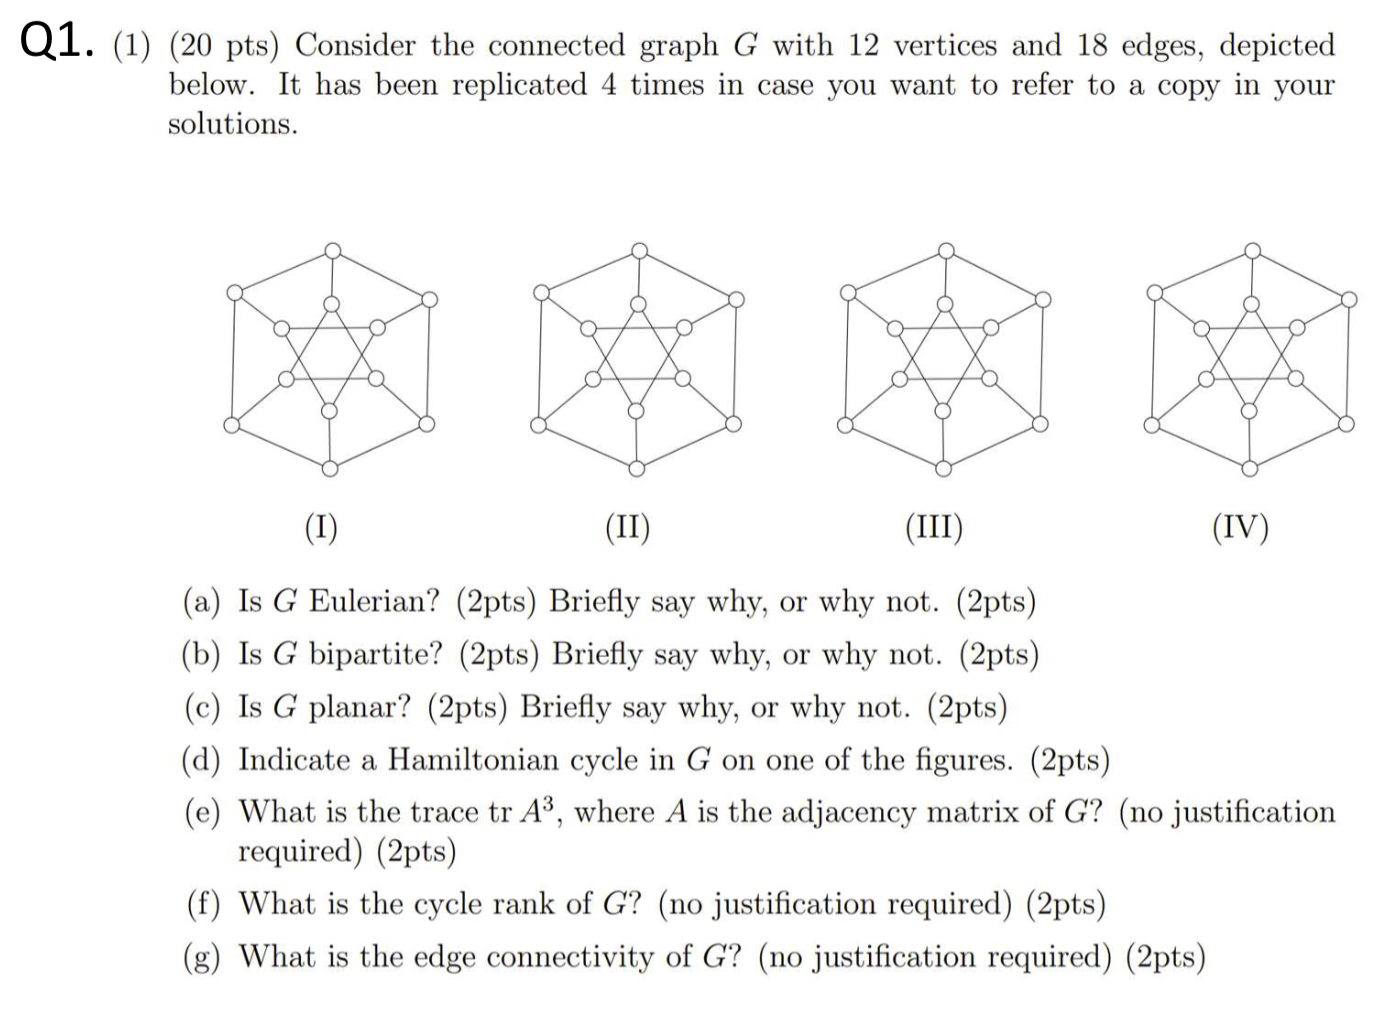
\includegraphics[width = 10 cm]{MockQ1.png}
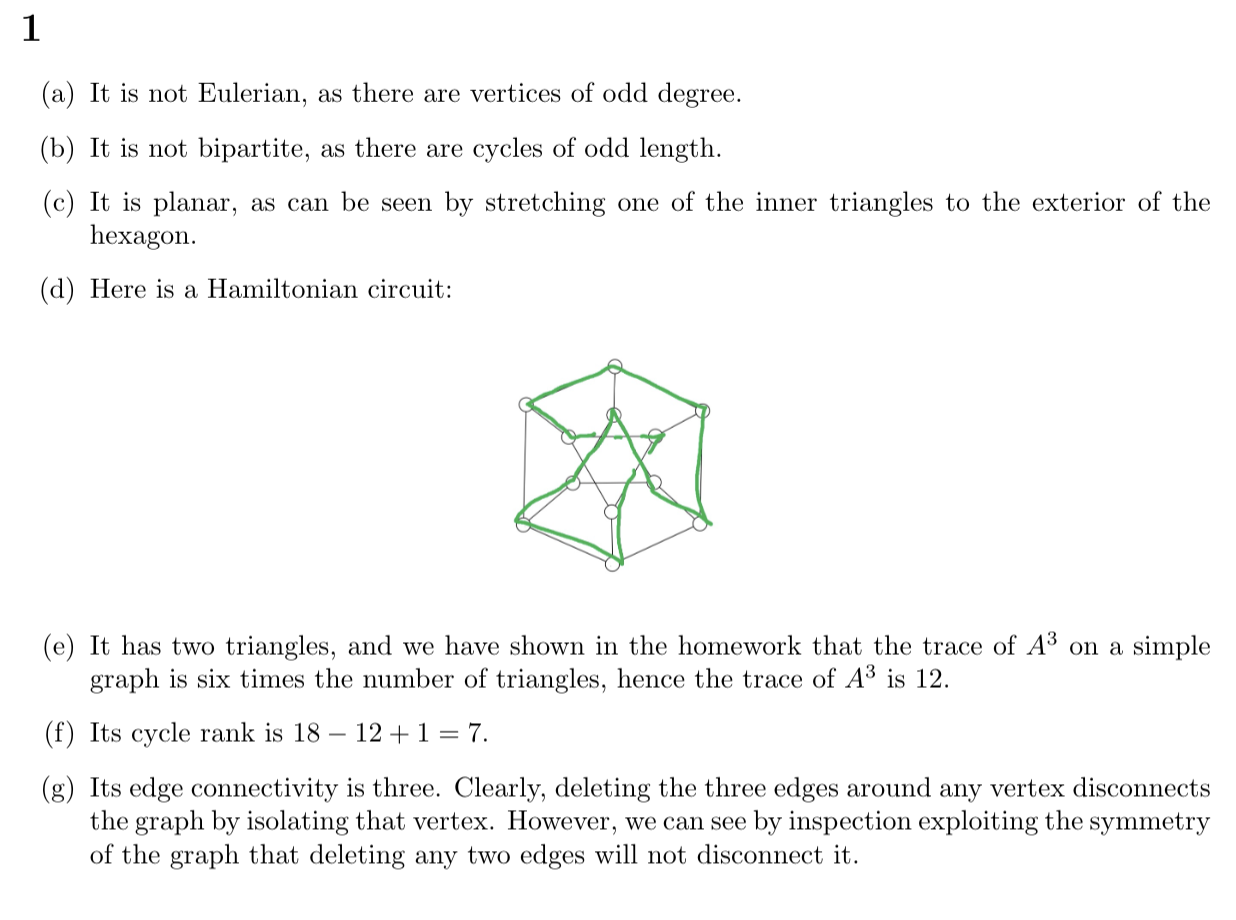
\includegraphics[width = 10 cm]{MockA1.png}
\newpage
\textbf{Dijkstra's, Guan's, Crit Path, T Salesman}
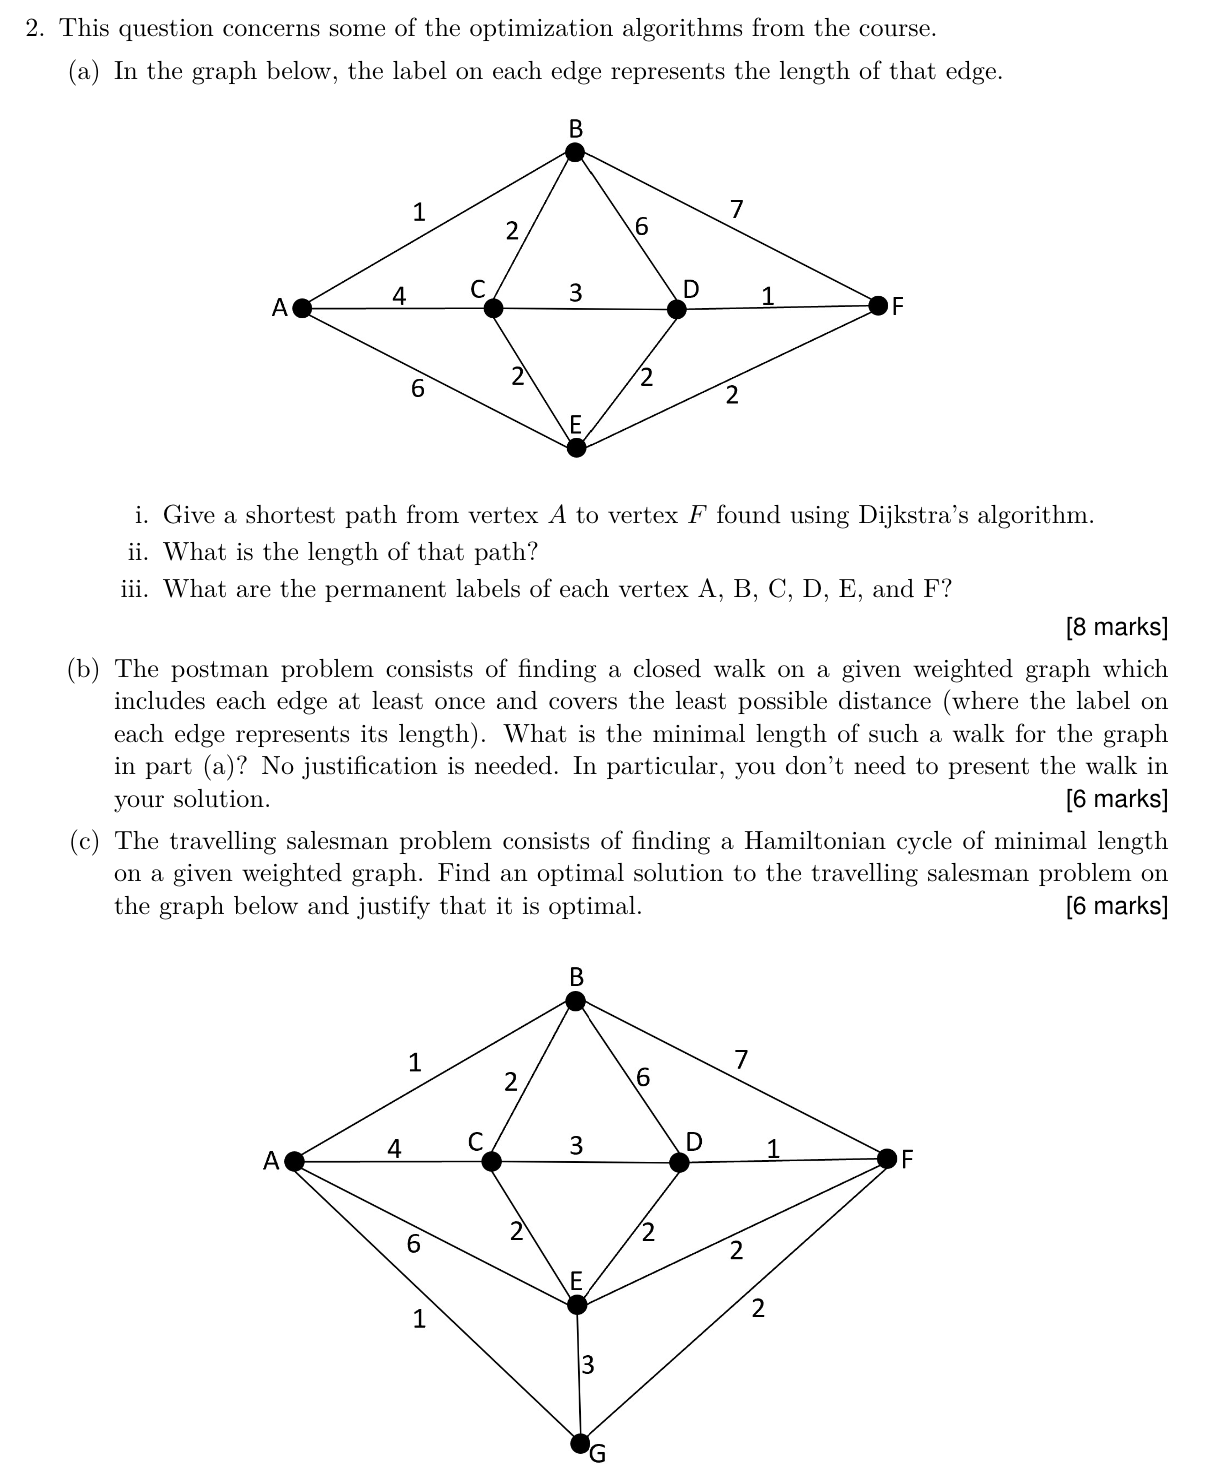
\includegraphics[width = 10 cm]{2023Q2.png}
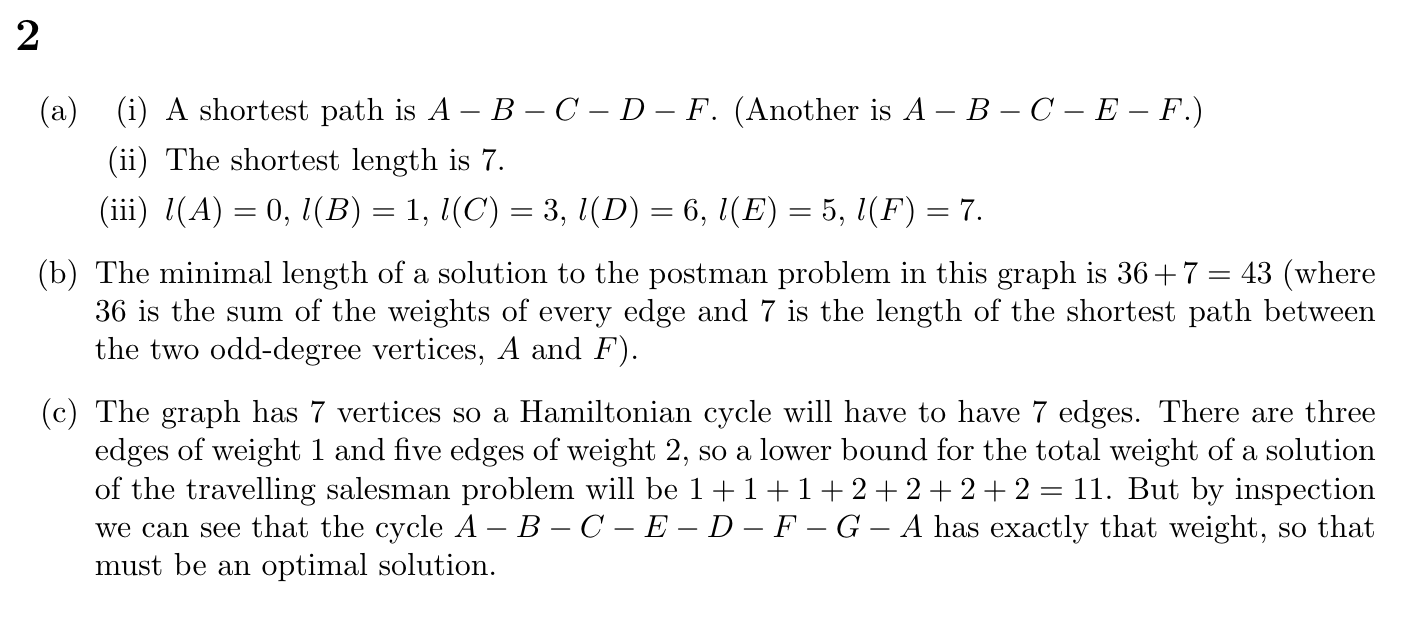
\includegraphics[width = 10 cm]{2023A2.png}\\
For the first one, use the following:
Start at A, set shortest path length to 0. \\
Then see where you can reach from A. We see that we can reach B, C and E. Update the Previous Node column (PN) in the table. This shows which node you were at before getting to the current one. Then pick the one with the shortest length. In our case this is B. Confirm B's permanent label SP = 1. See where we can get to from B and update the table. We see we can get to C from A in 1 less going via B. This is now the shortest path to C. Update the table and then pick the next smallest number. Continue this until you have covered all vertices, where the final iteration of the table shows the permanent labels of each vertex.\\
\vspace{0.2cm}
\begin{tabular}{ |c|c|c| } 
\hline
N & SP & PN \\
\hline
A & 0 $\checkmark$ &  \\ 
B & 1 & A \\ 
C & 4 & A \\ 
D &  &  \\ 
E & 6 & A \\ 
F &  &  \\
\hline
\end{tabular}
\begin{tabular}{ |c|c|c| } 
\hline
N & SP & PN \\
\hline
A & 0 &  \\ 
B & 1 $\checkmark$ & A \\ 
C & 3 & B \\ 
D & 7 & B \\ 
E & 6 & A \\ 
F & 8 & B \\
\hline
\end{tabular}
\begin{tabular}{ |c|c|c| } 
\hline
N & SP & PN \\
\hline
A & 0 $\checkmark$ &  \\ 
B & 1 $\checkmark$ & A \\ 
C & 3 $\checkmark$ & B \\ 
D & 6 & C \\ 
E & 5 & C \\ 
F & 8 & B \\
\hline
\end{tabular}
\begin{tabular}{ |c|c|c| } 
\hline
N & SP & PN \\
\hline
A & 0 $\checkmark$ &  \\ 
B & 1 $\checkmark$ & A \\ 
C & 3 $\checkmark$ & B \\ 
D & 6 $\checkmark$ & C \\ 
E & 5 $\checkmark$ & C \\ 
F & 7 $\checkmark$ & E or D \\
\hline
\end{tabular}
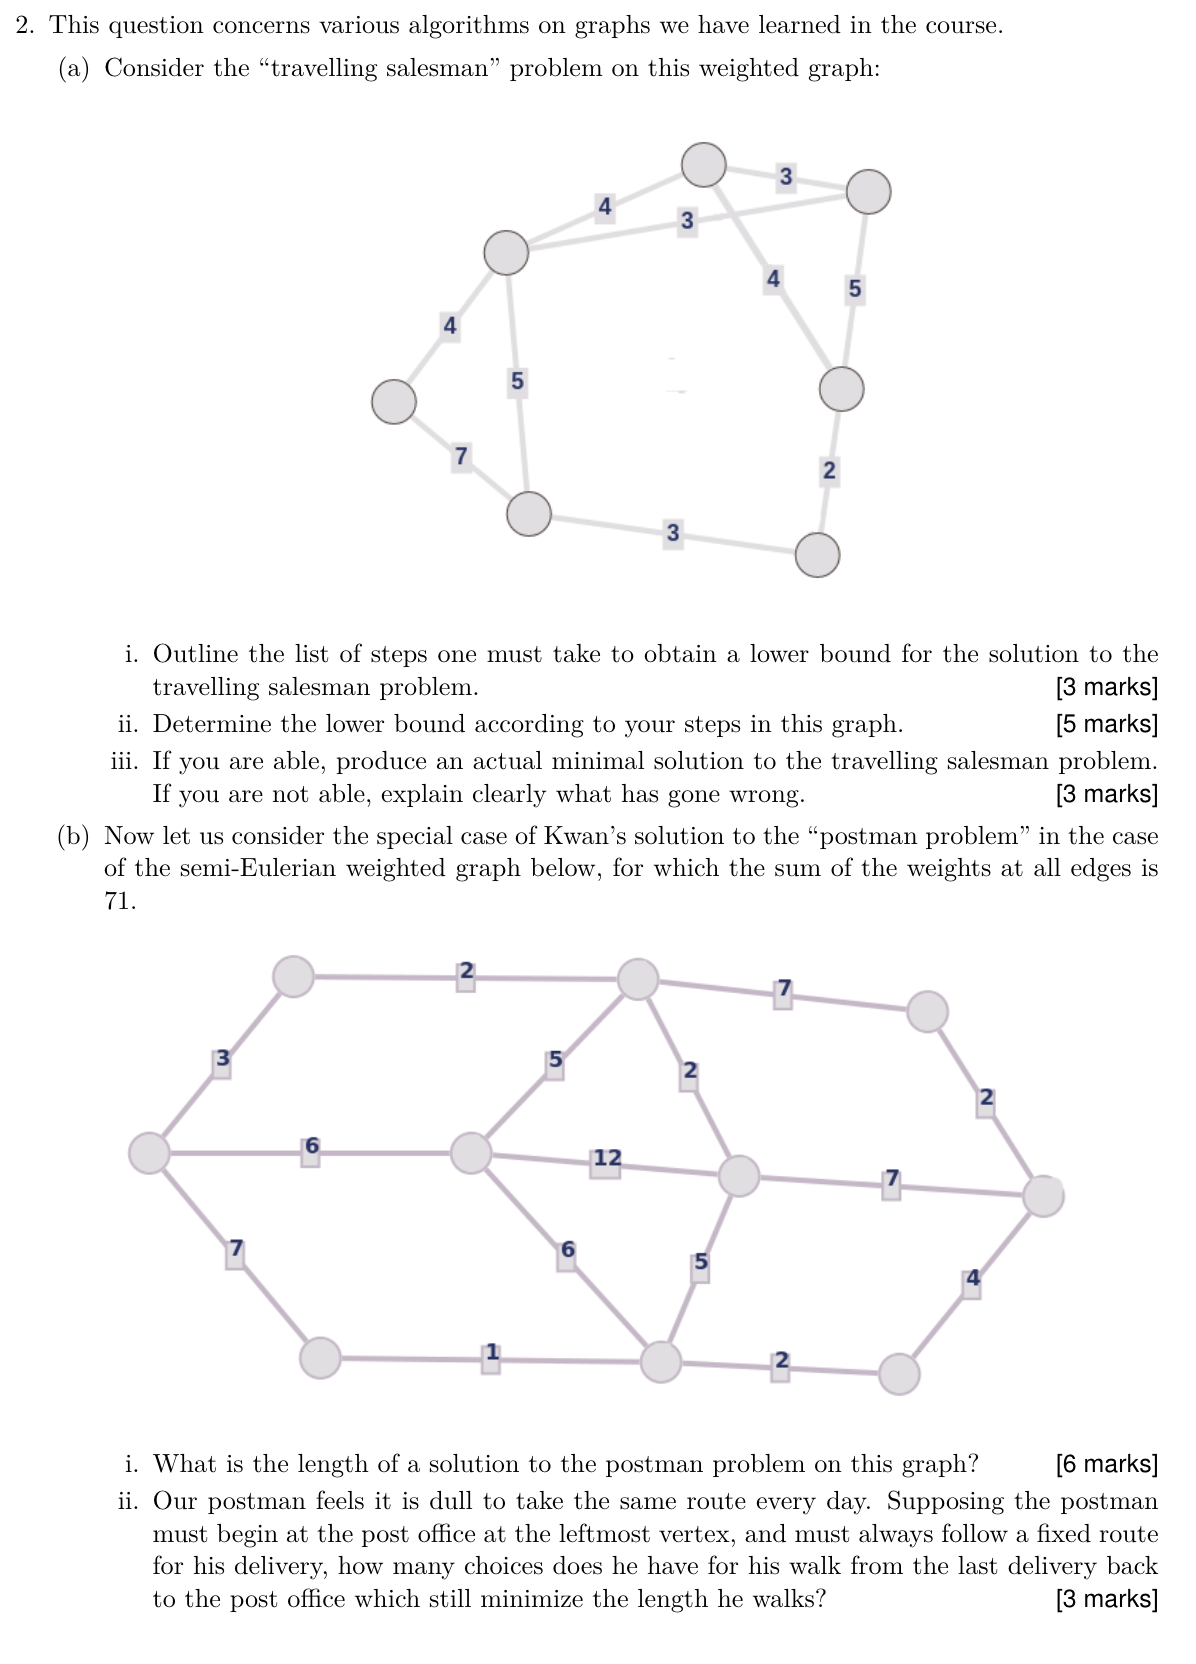
\includegraphics[width = 9 cm]{2022Q2.png}
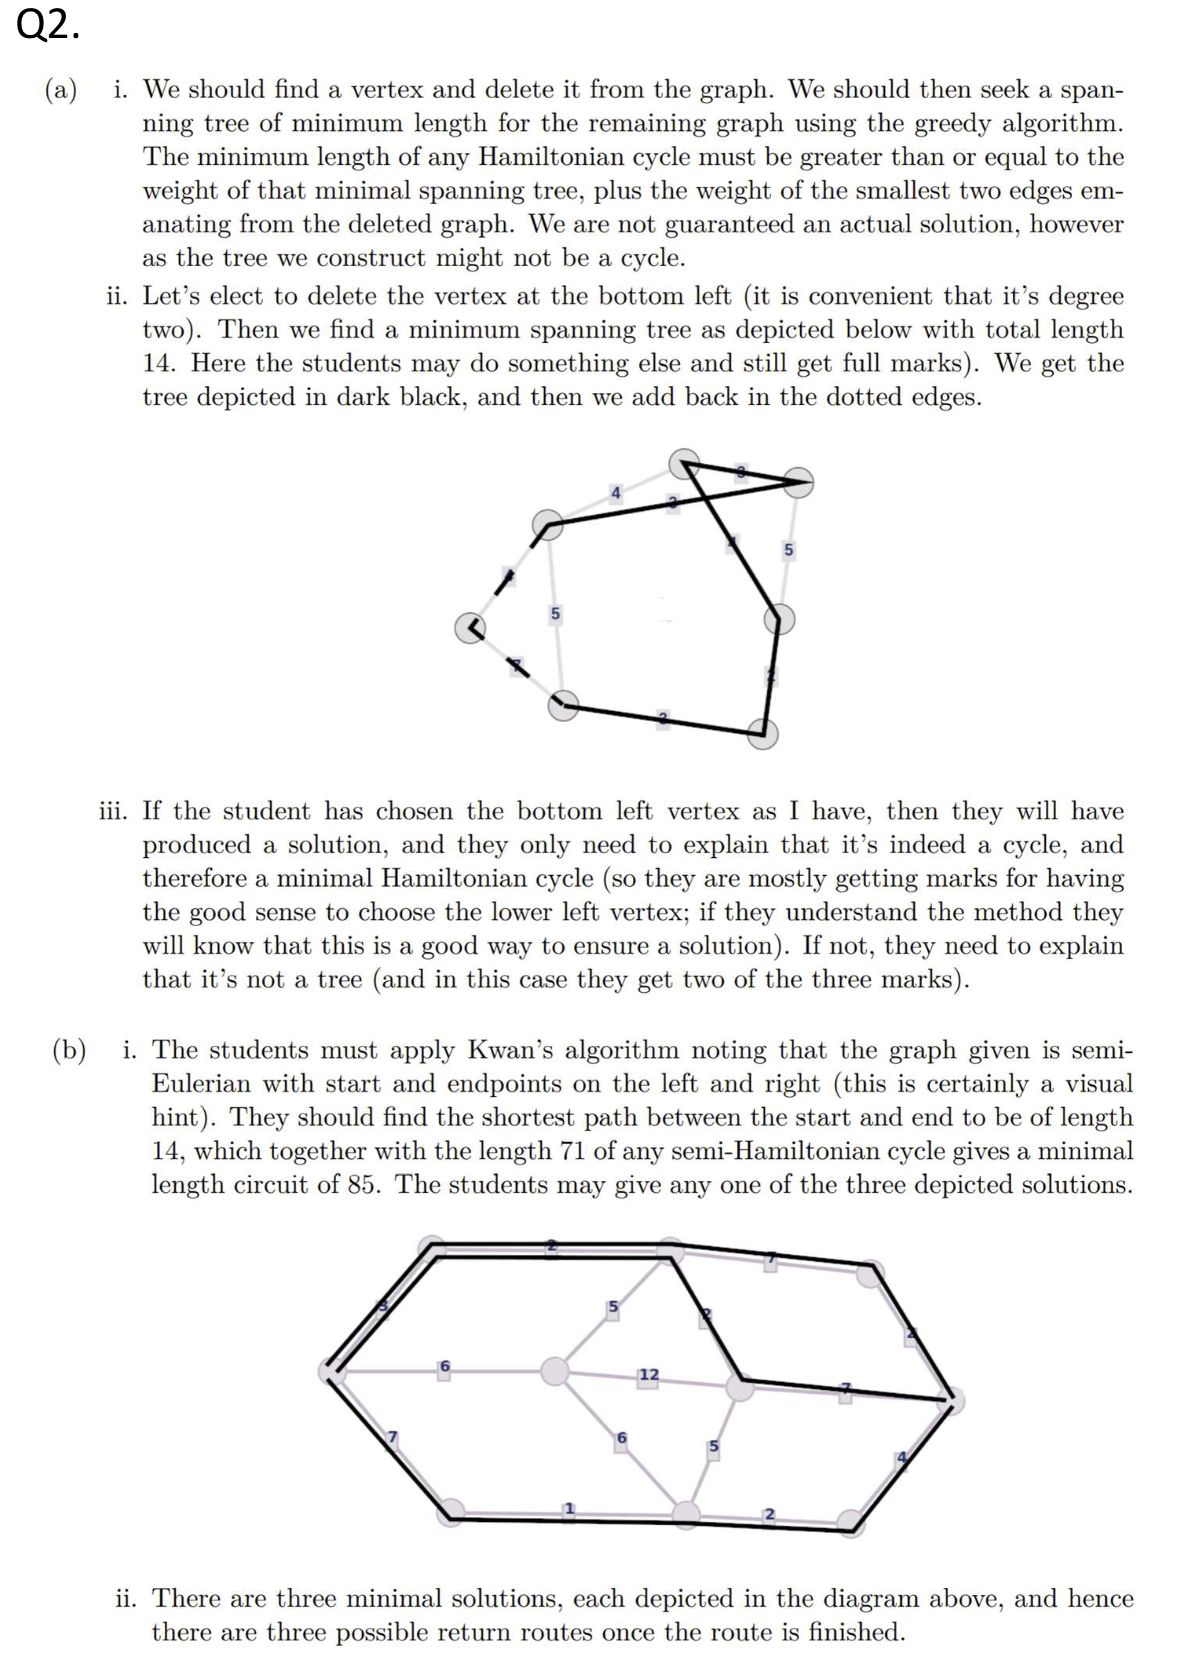
\includegraphics[width = 9 cm]{2022A2.png}
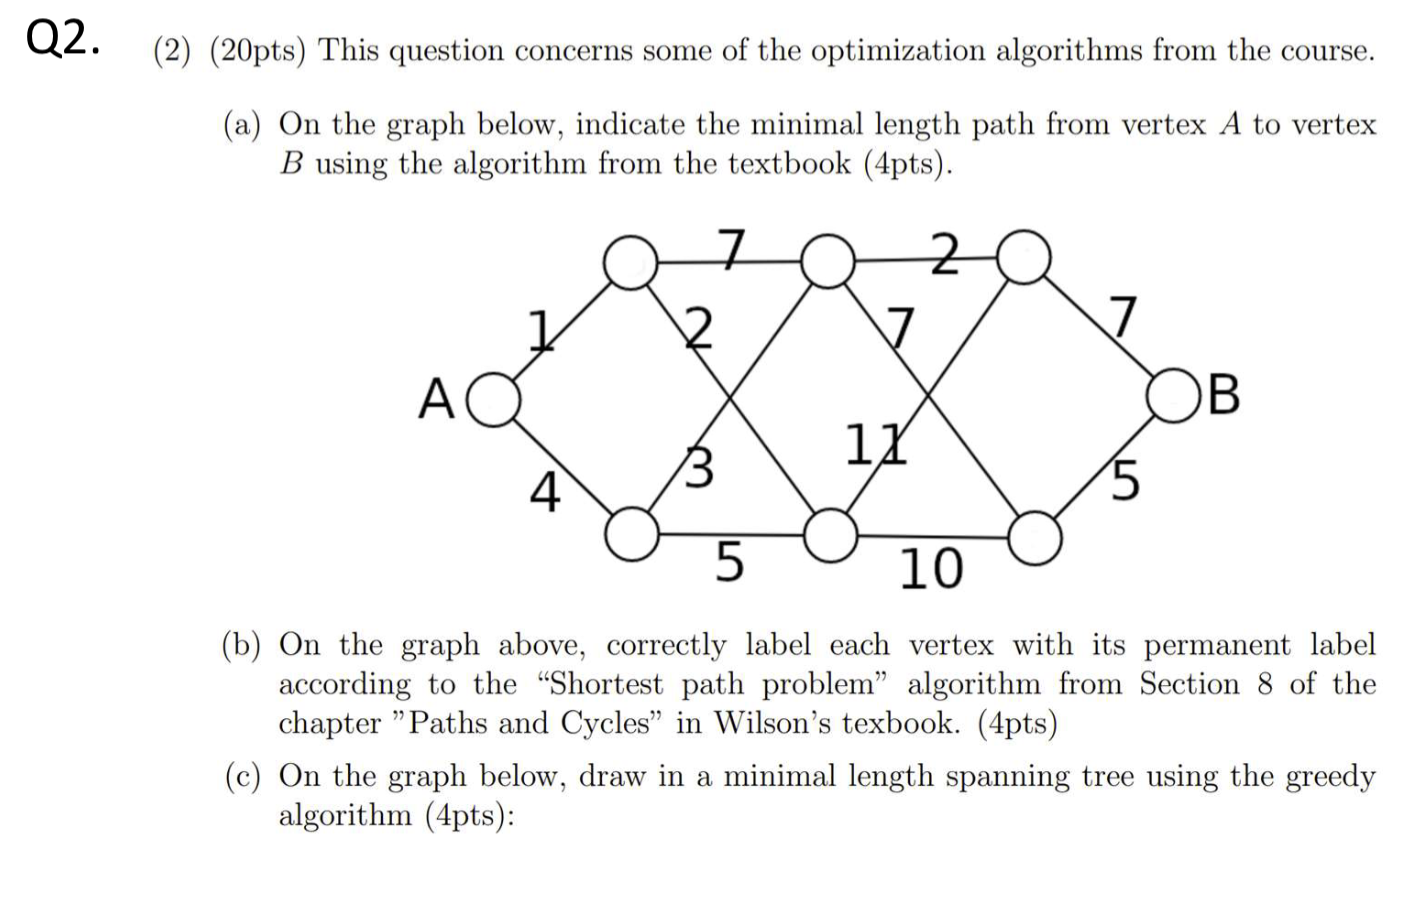
\includegraphics[width = 9 cm]{MockQ2p1.png}
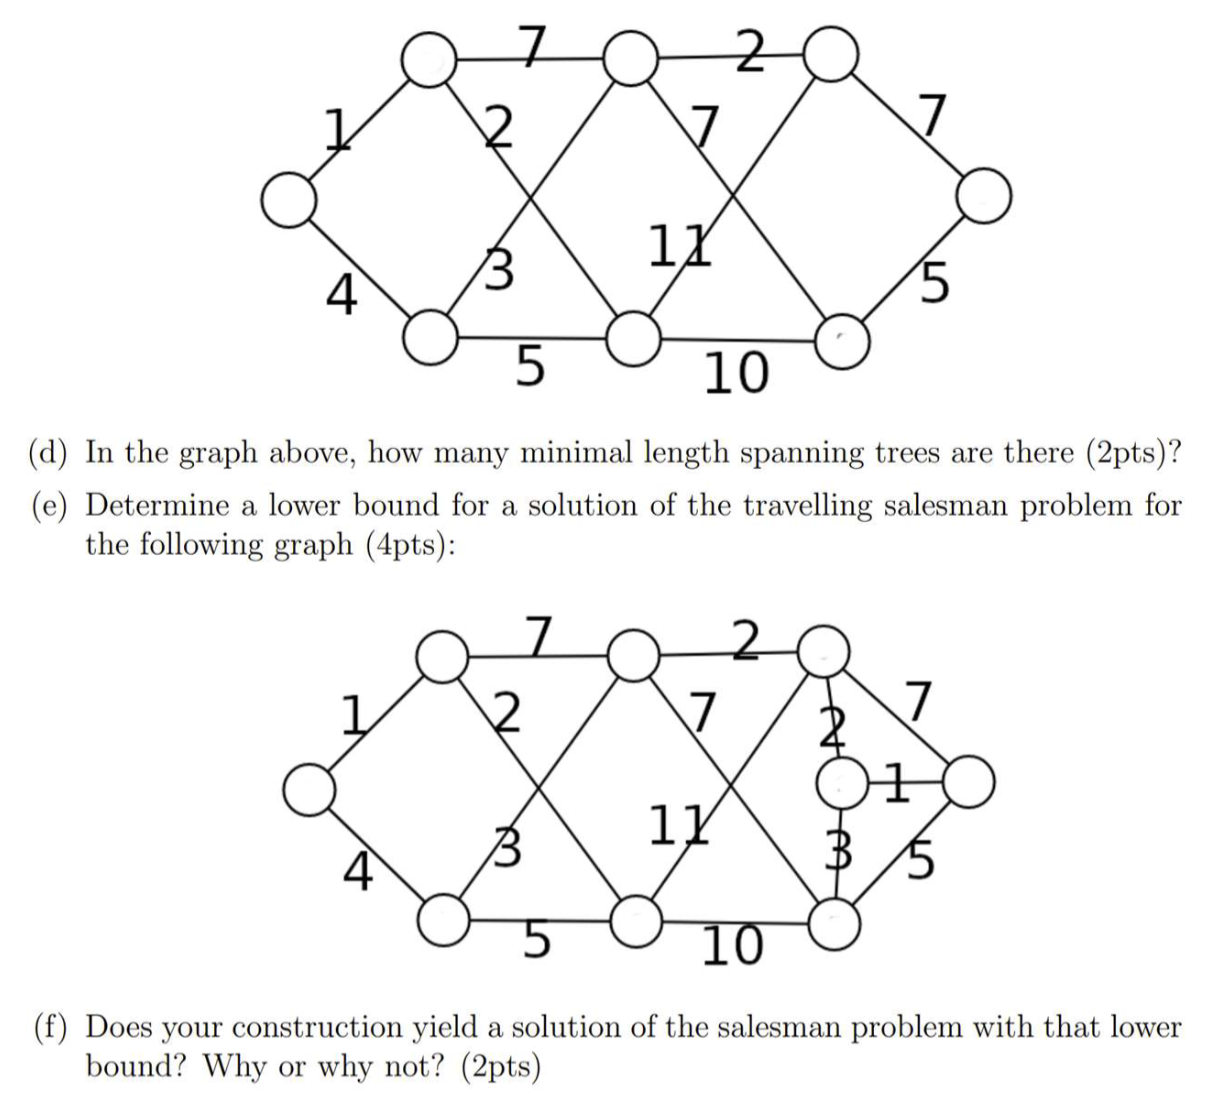
\includegraphics[width = 9 cm]{MockQ2p2.png}
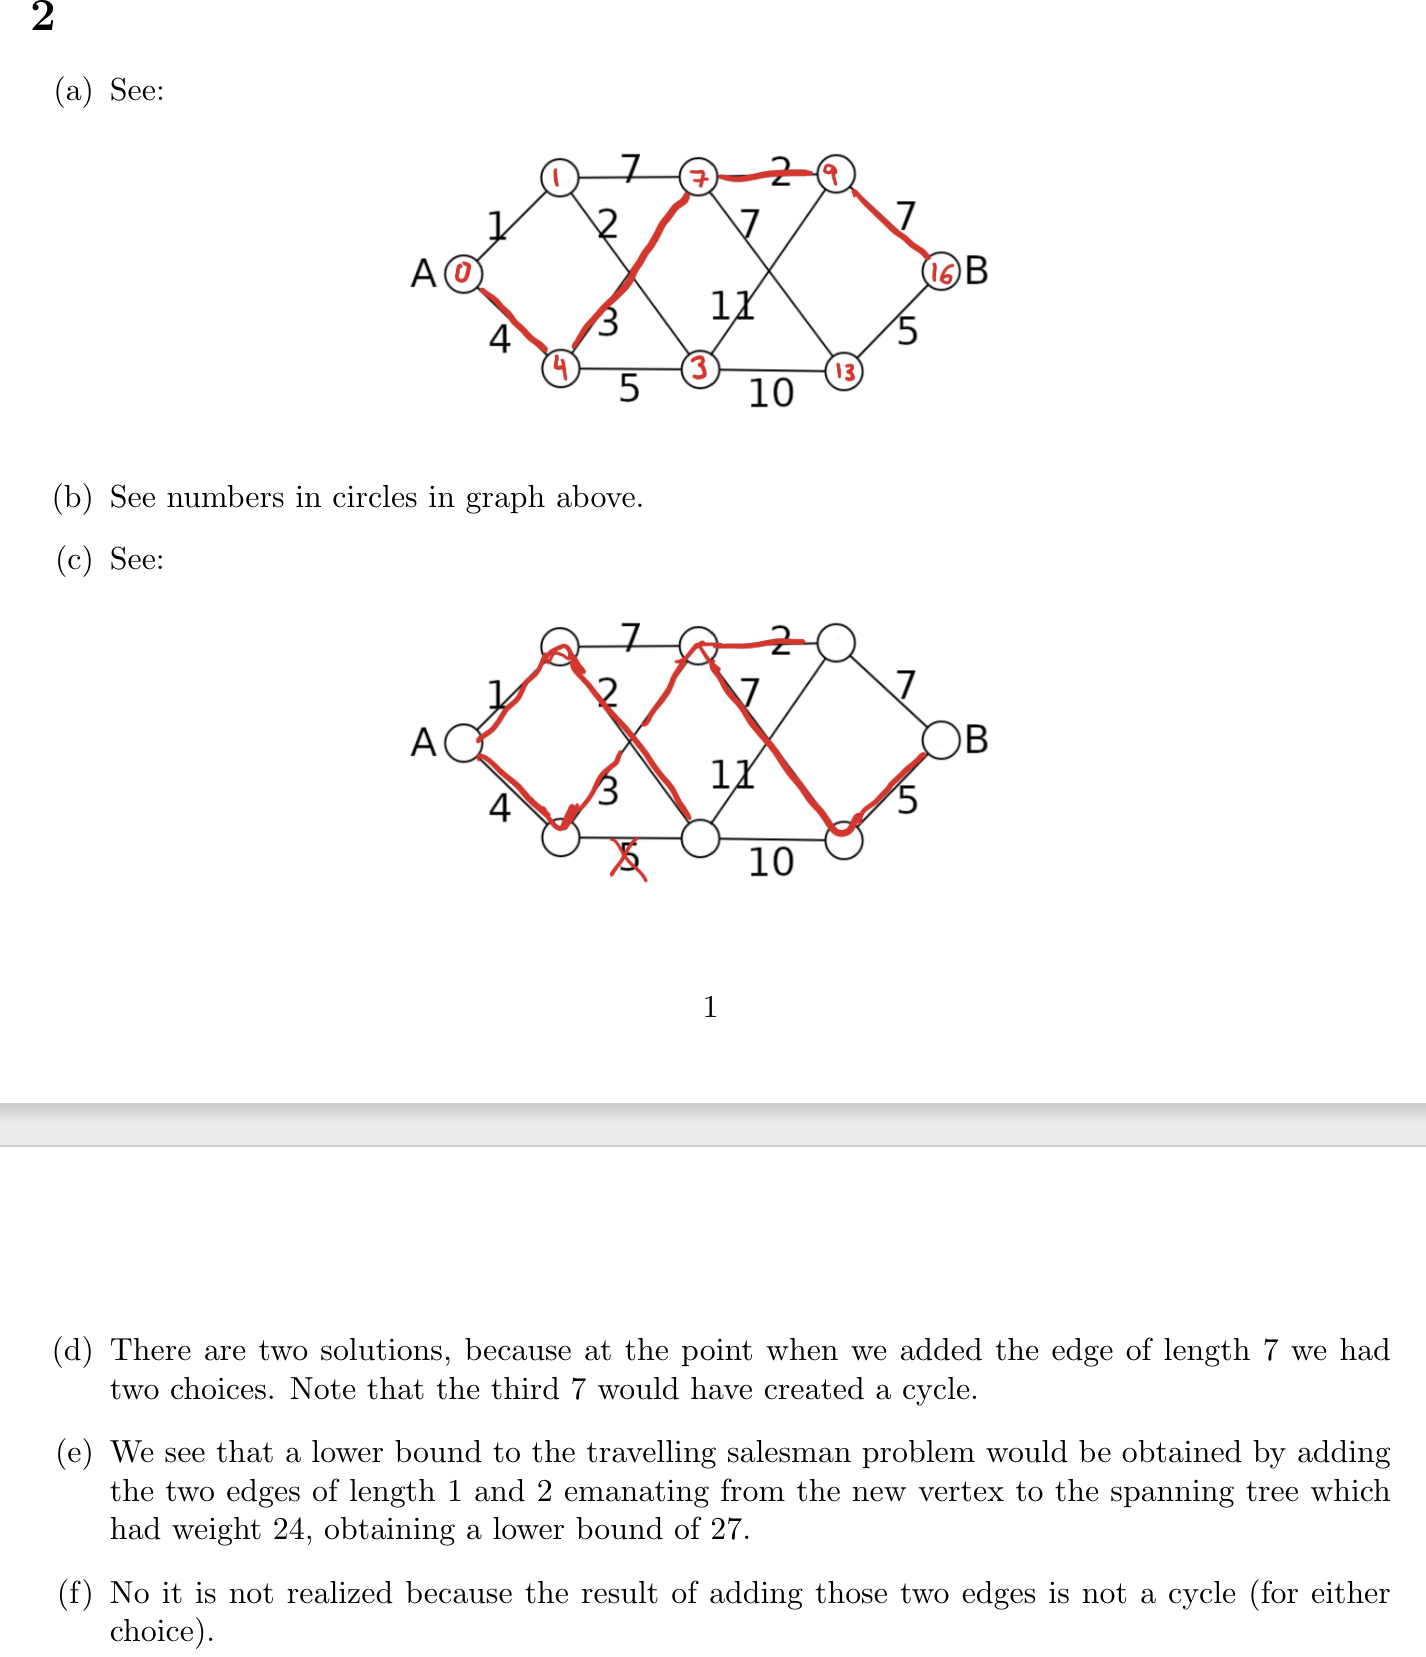
\includegraphics[width = 9 cm]{MockA2.png}
\textbf{Chromatic Polynomials + Trees etc}

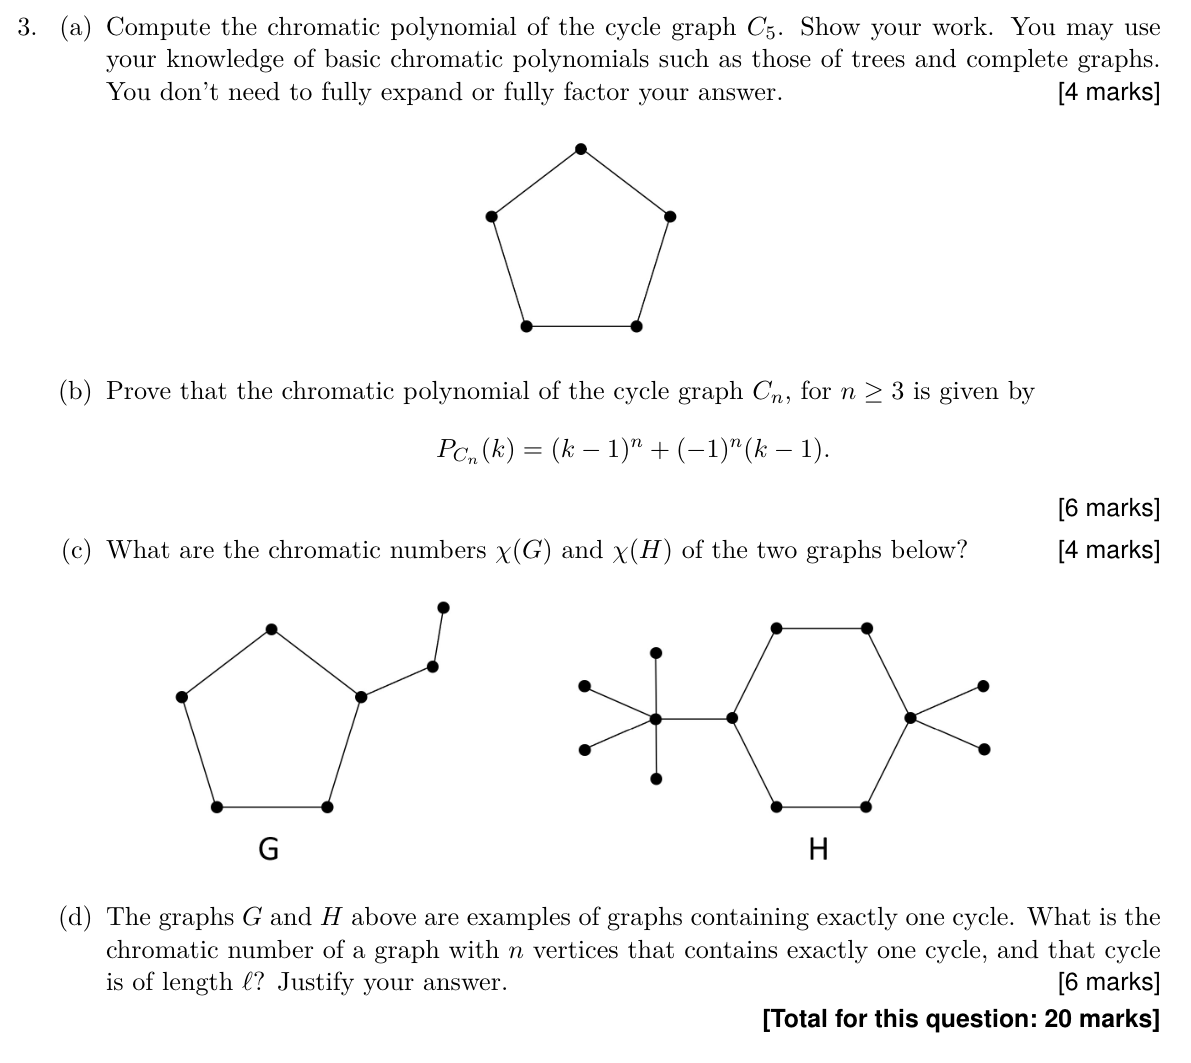
\includegraphics[width = 10 cm]{2023Q3.png}
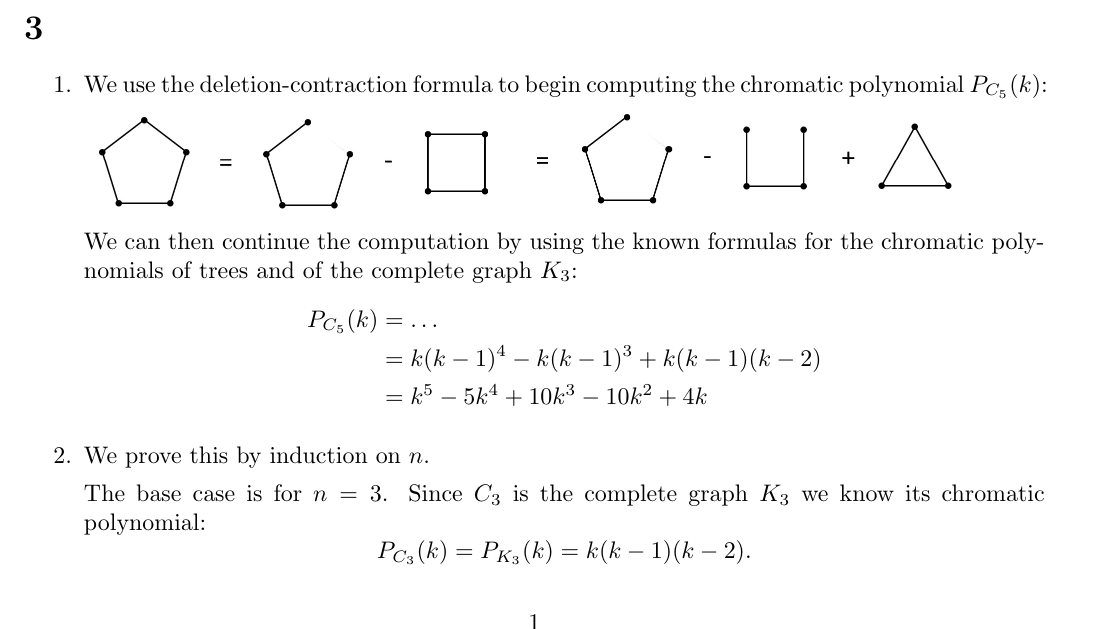
\includegraphics[width = 10 cm]{2023A3p1.png}
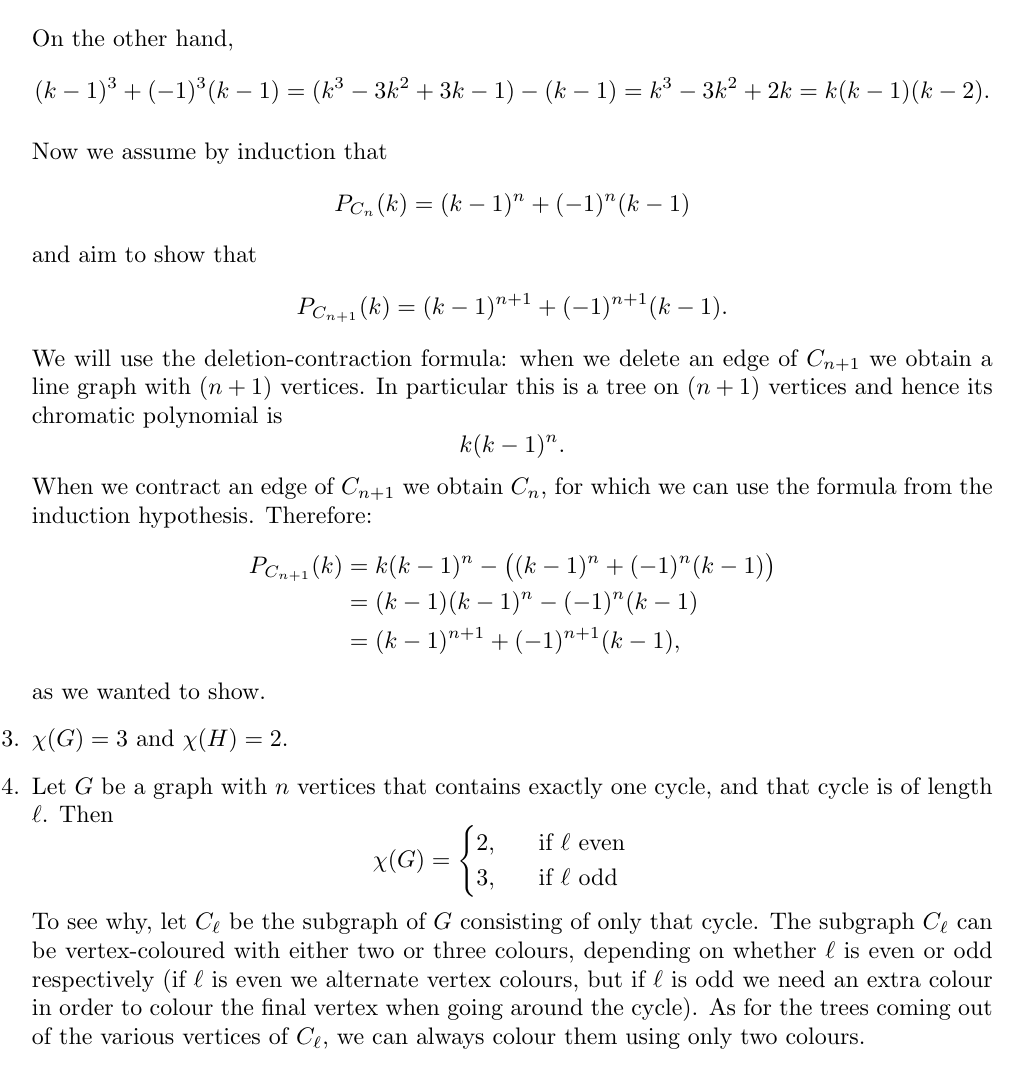
\includegraphics[width = 10 cm]{2023A3p2.png}
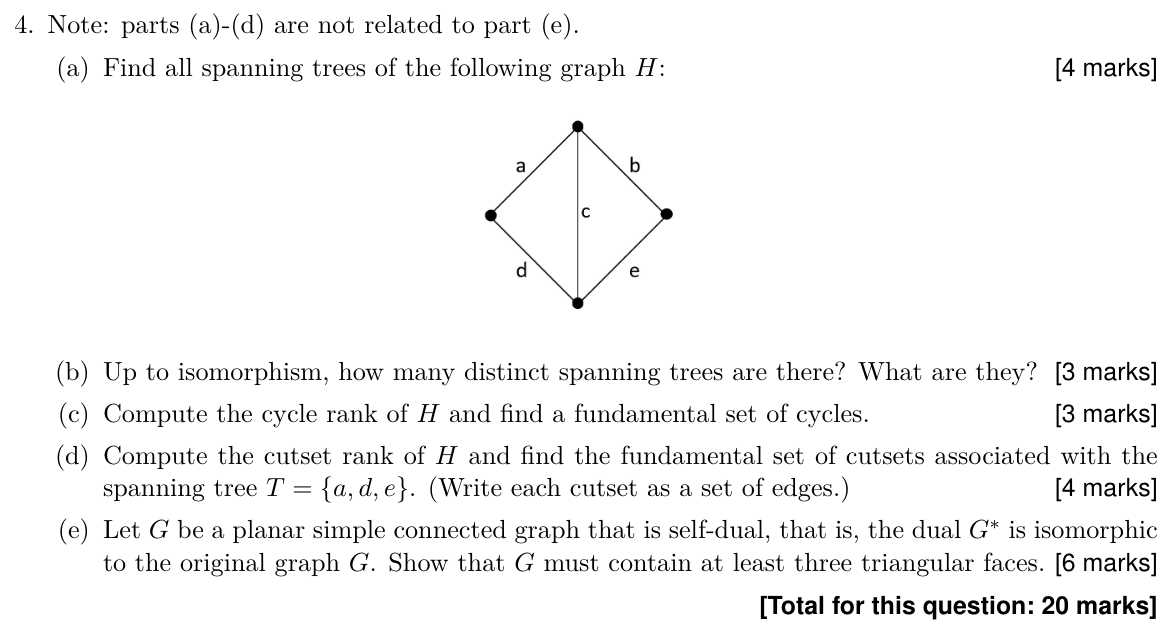
\includegraphics[width = 9.5 cm]{2023Q4.png}
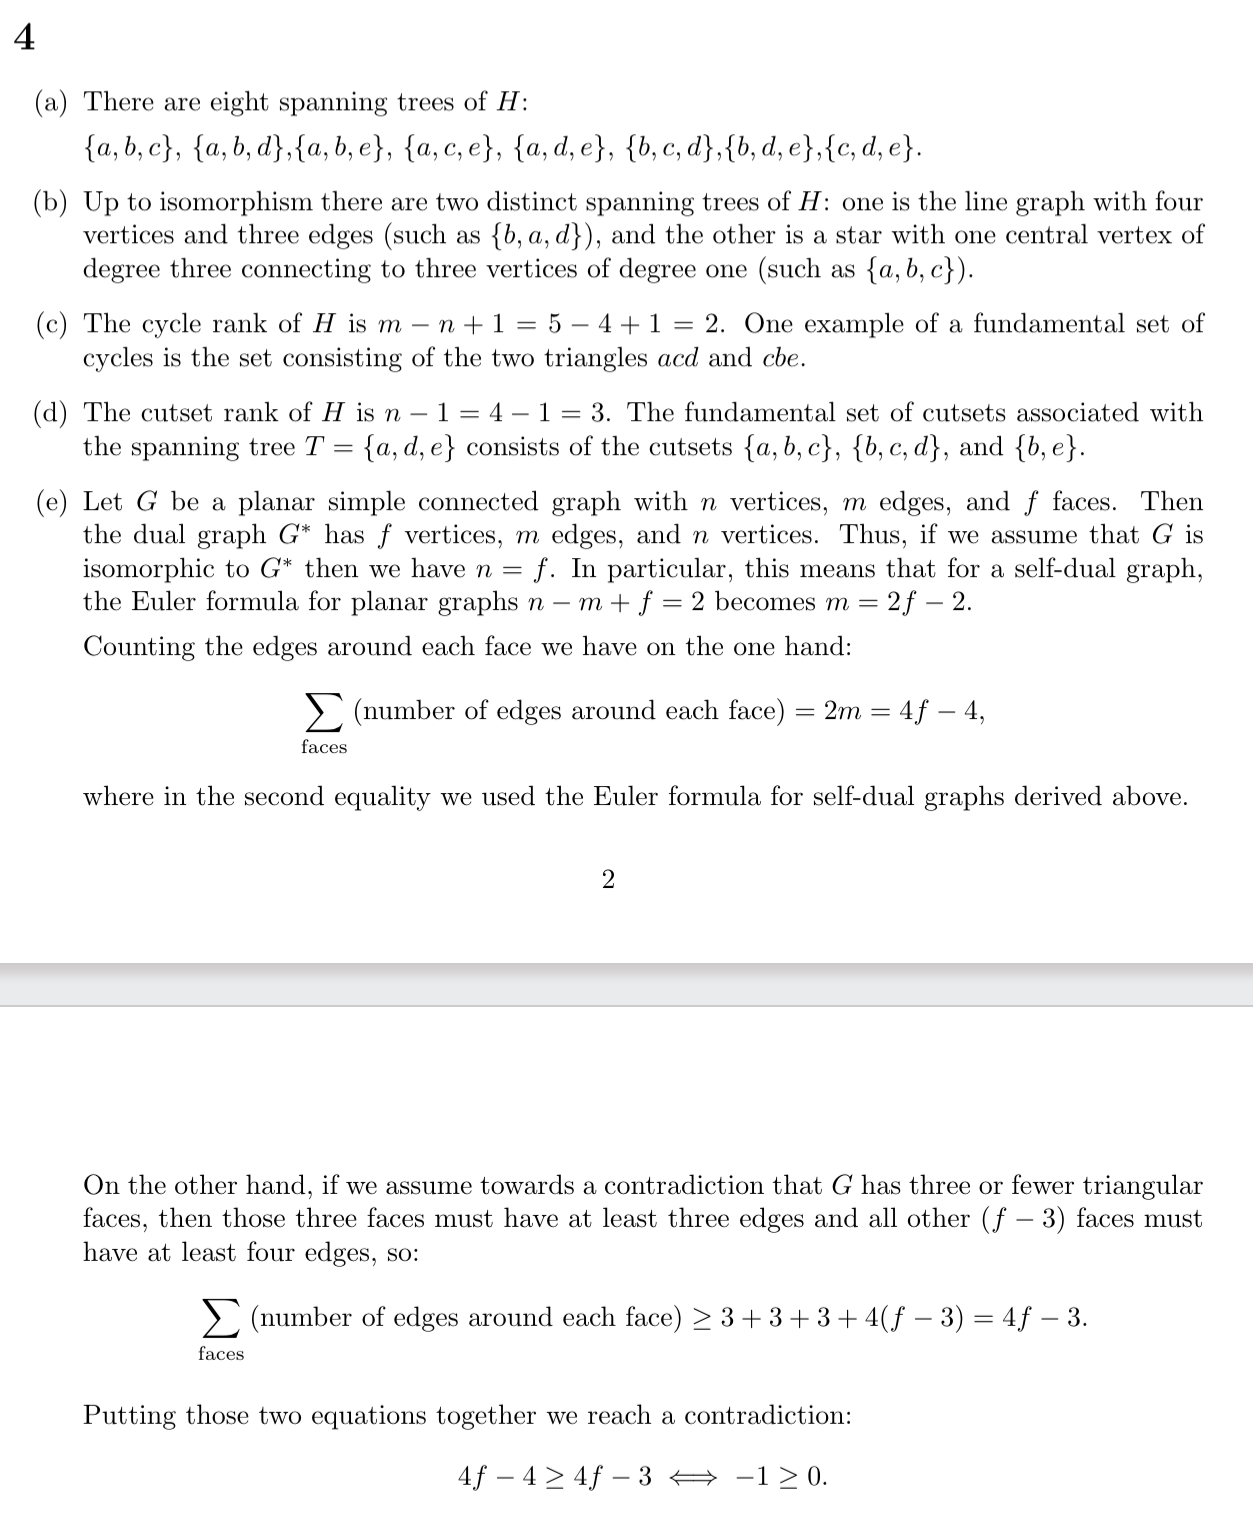
\includegraphics[width = 9.5 cm]{2023A4.png}
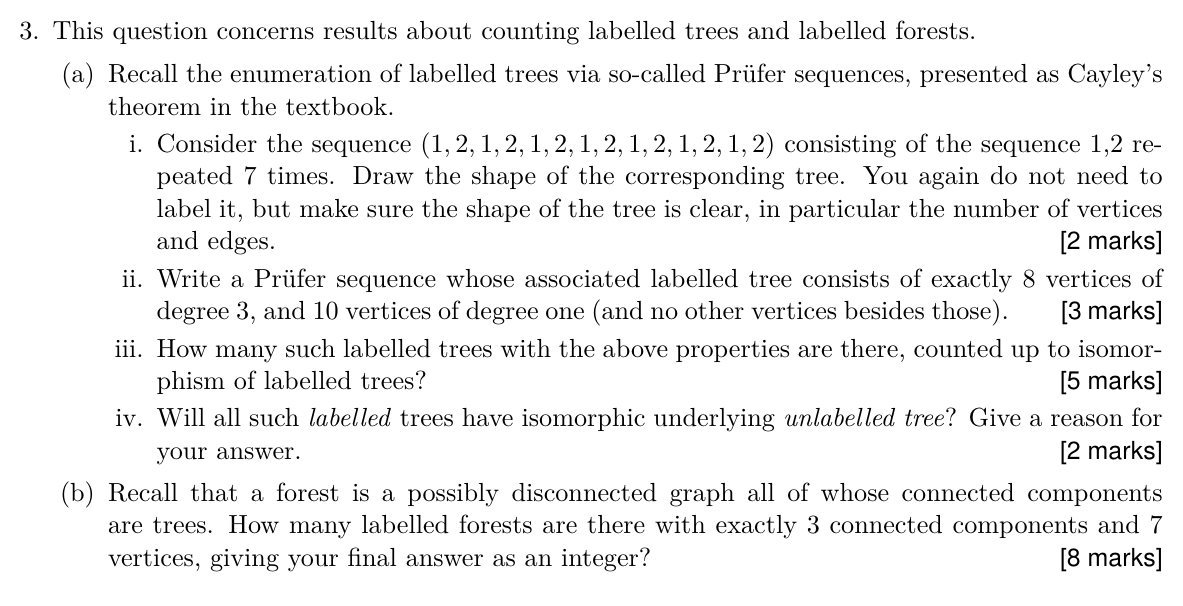
\includegraphics[width = 9.5 cm]{2022Q3_Prufer.png}
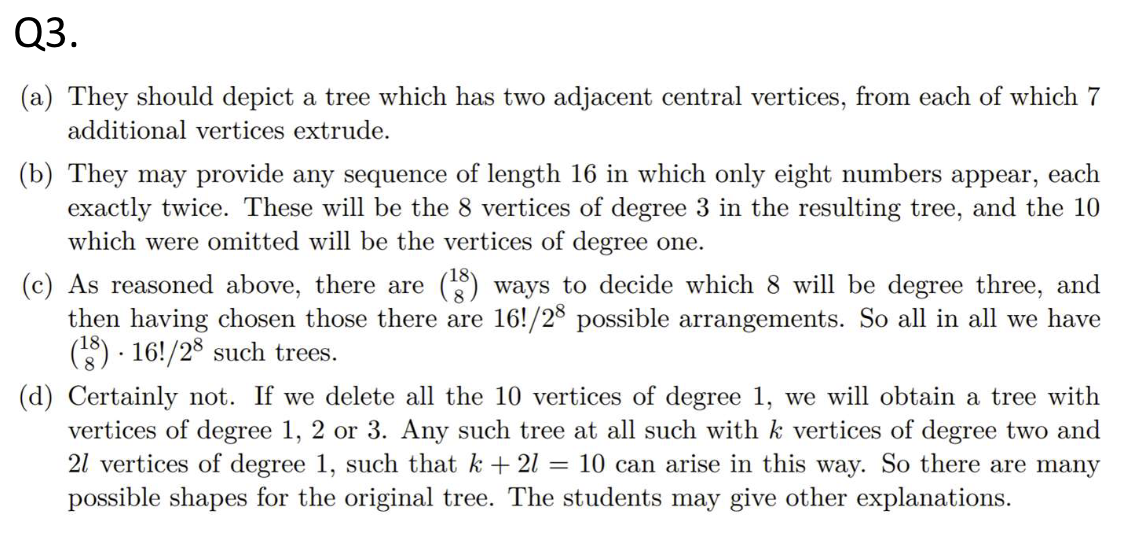
\includegraphics[width = 10 cm]{2022A3.png}
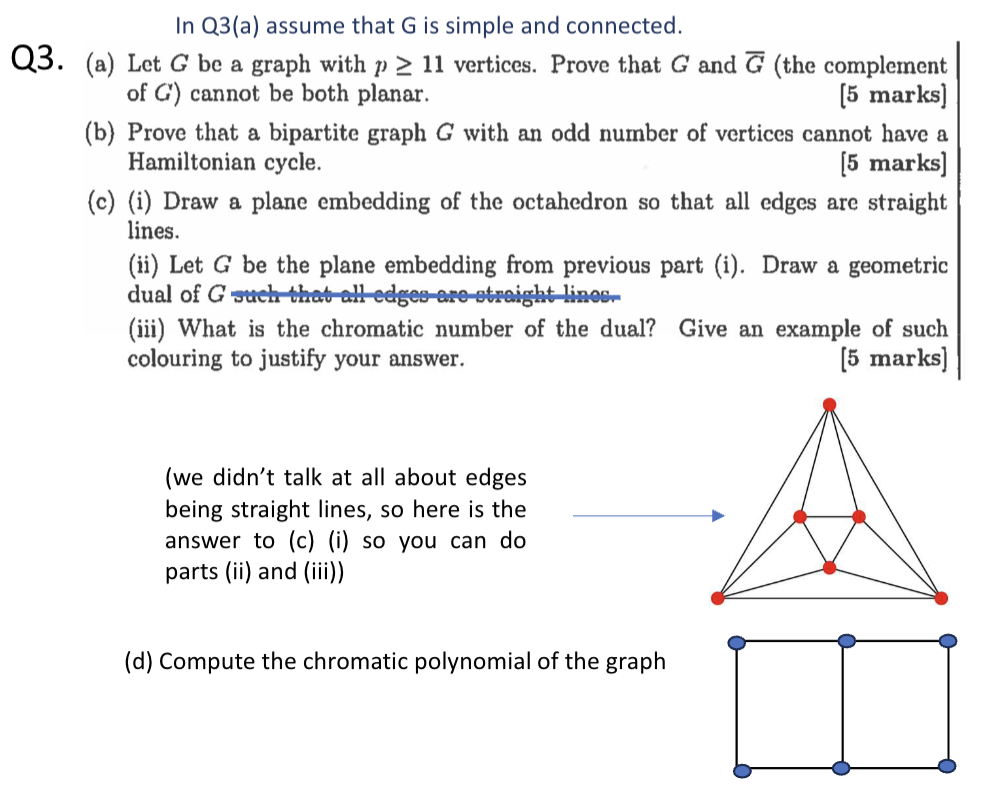
\includegraphics[width = 9.5 cm]{MockQ3.png}
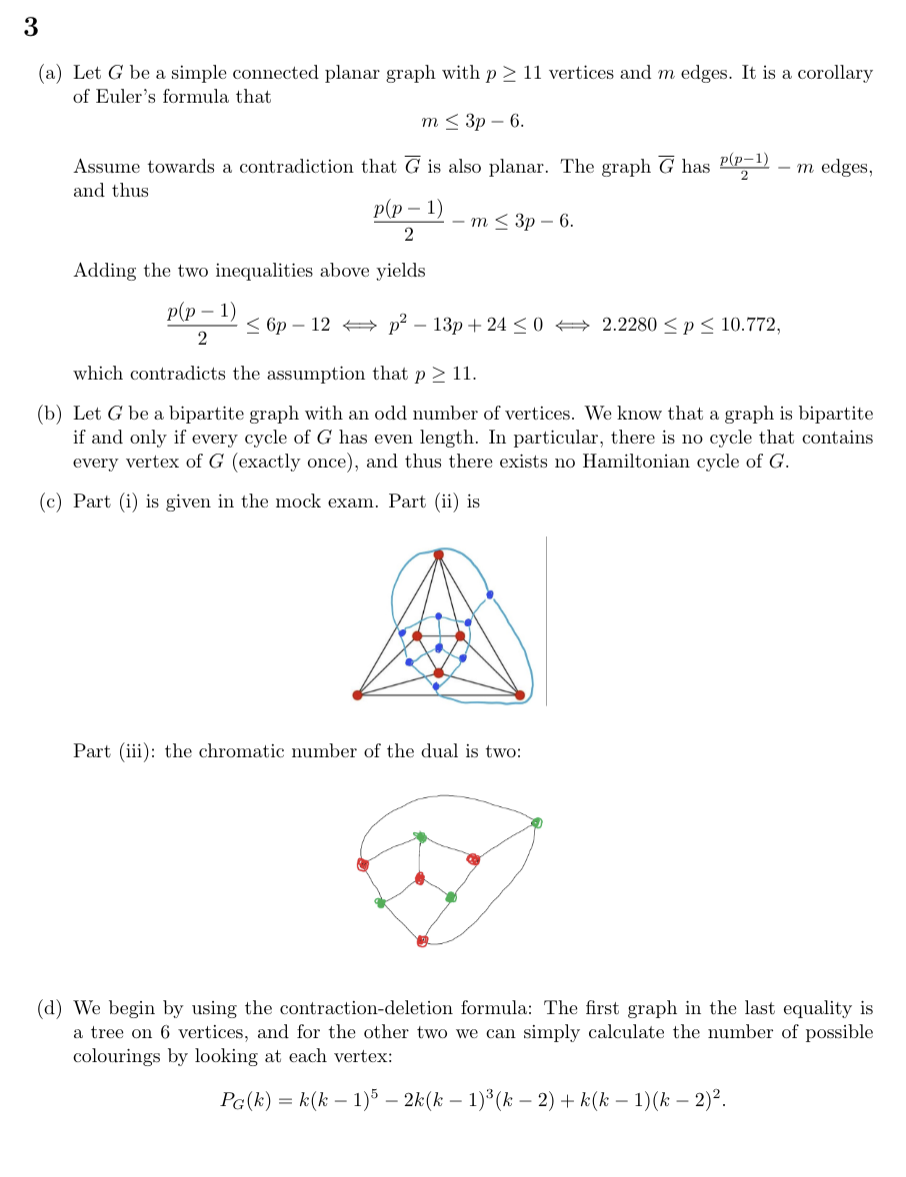
\includegraphics[width = 10.2 cm]{MockA3p1.png}
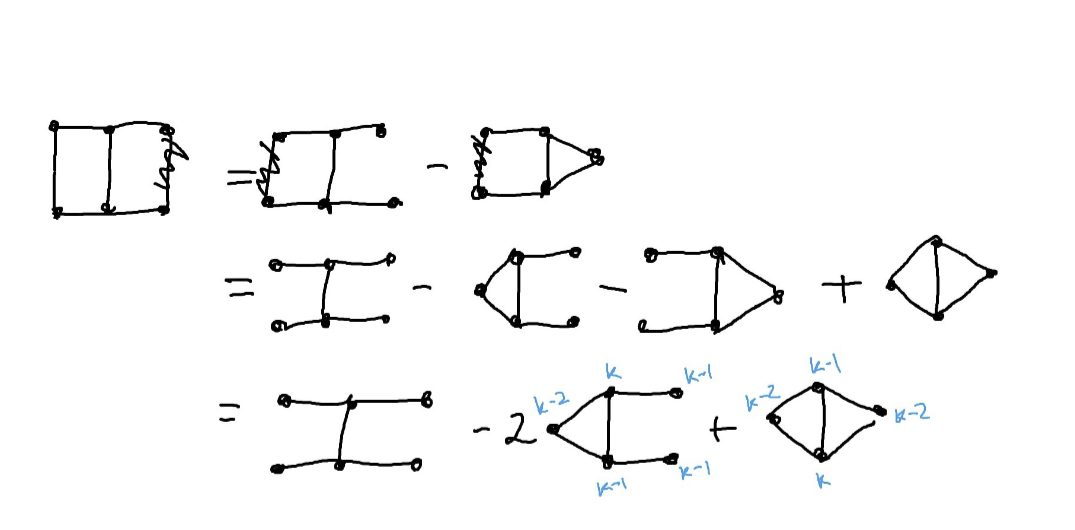
\includegraphics[width = 10 cm]{MockA3p2.png}
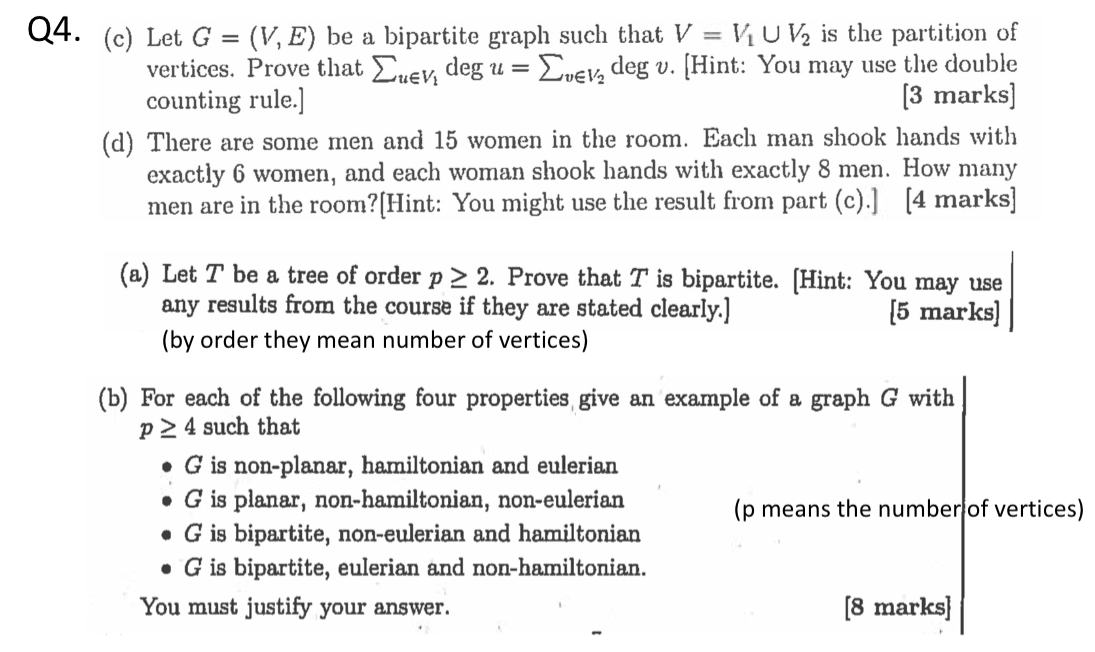
\includegraphics[width = 10 cm]{MockQ4.png}
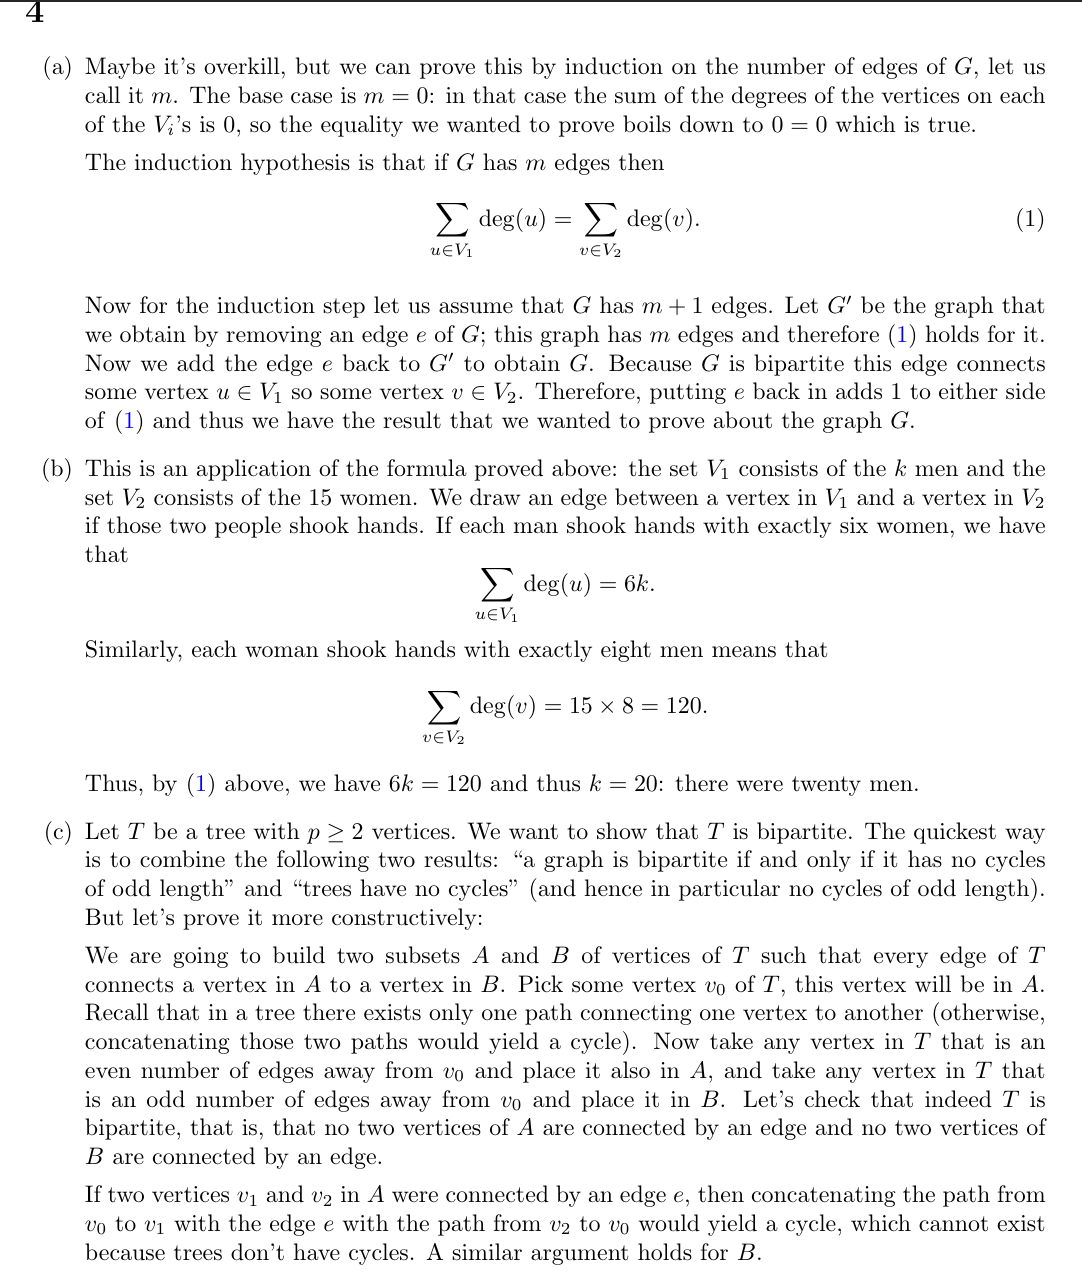
\includegraphics[width = 10 cm]{MockA4p1.png}
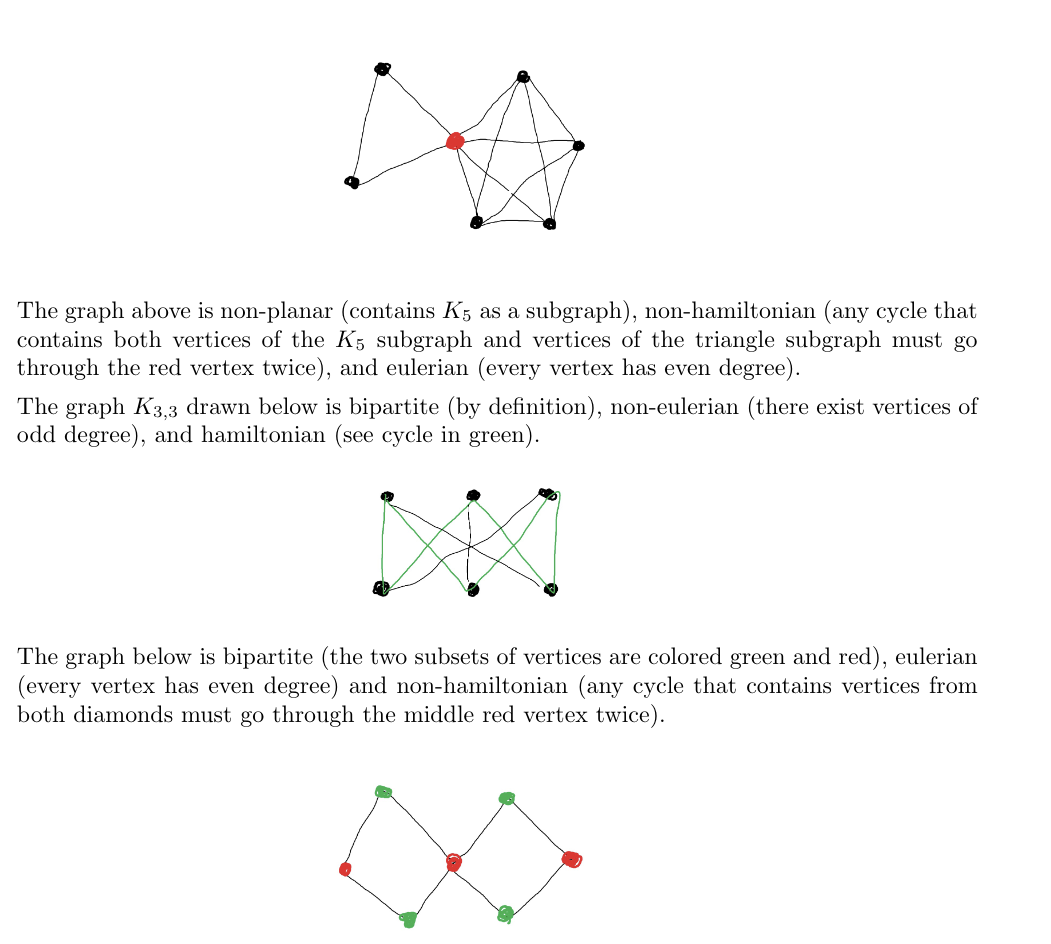
\includegraphics[width = 10 cm]{MockA4p2.png}

\textbf{Miscellaneous + End Proofs}
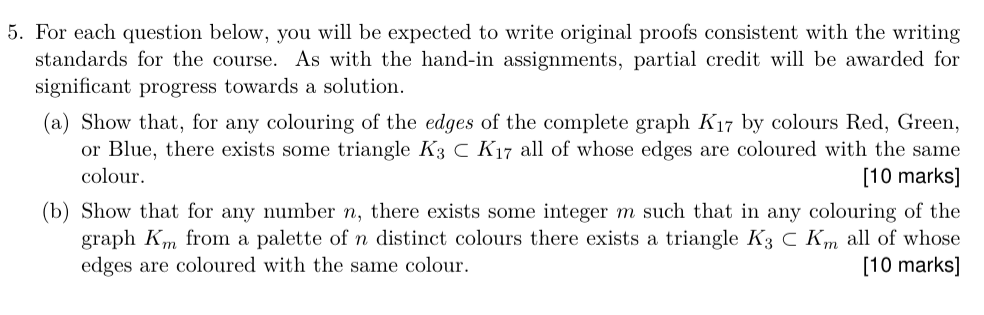
\includegraphics[width = 9.5 cm]{2022Q5.png}
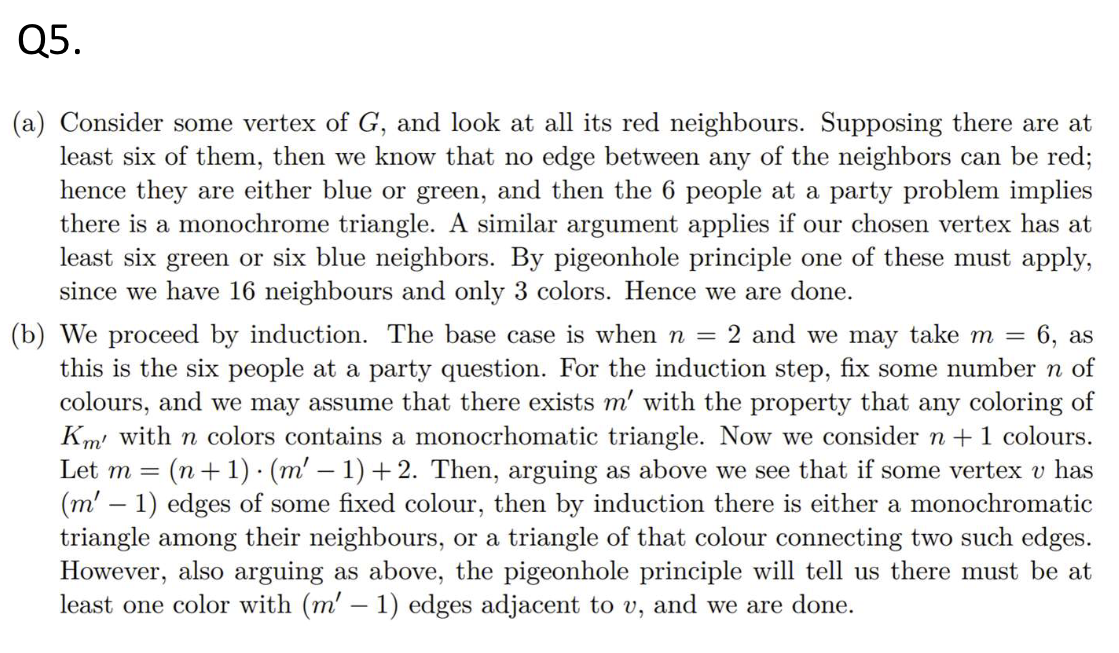
\includegraphics[width = 9.5 cm]{2022A5.png}
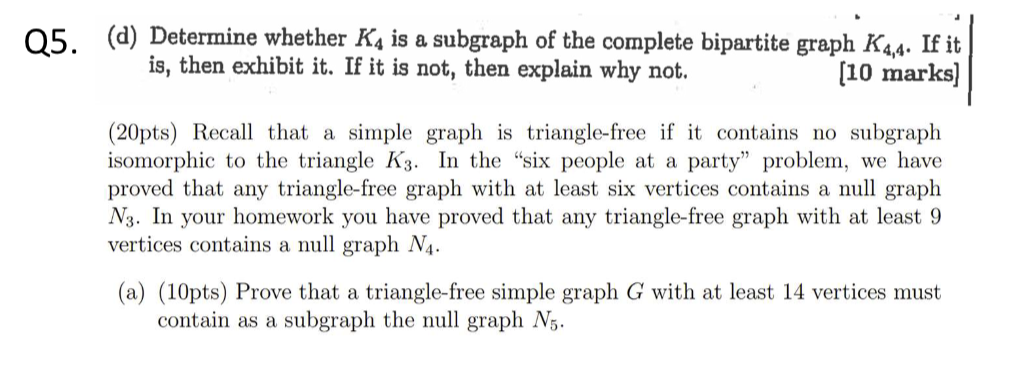
\includegraphics[width = 9.5 cm]{MockQ5.png}
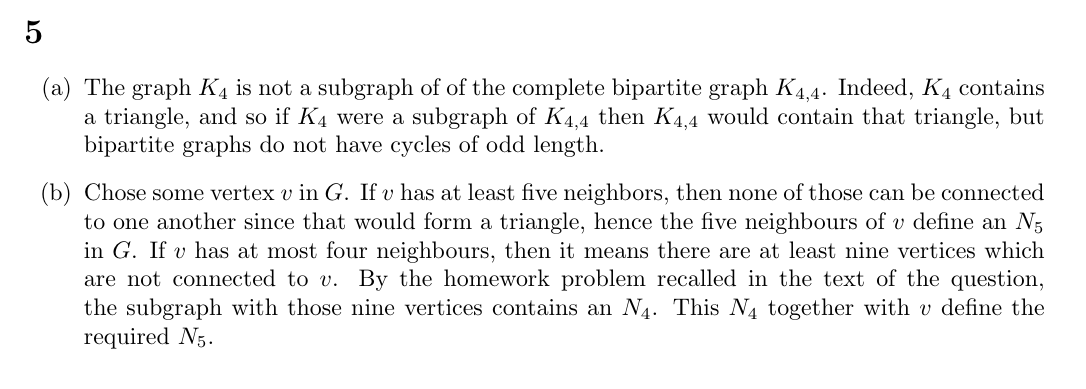
\includegraphics[width = 9.5 cm]{MockA5.png}




\scriptsize

\textbf{Other}

\textbf{1.10:} Show that there are exactly $n^{n(n-1)/2}$ labelled simple graphs on $n$ vertices.

\textbf{Proof:} We proceed by induction
\begin{itemize}
    \item Base Case: $n=2$

    We start with $n=2$ since there are no simple graphs with less than 2 vertices that can be labelled differently. using this we obtain: $2^{n(n-1)/2}=2^{2(2-1)/2} = 2^1 = 2$. The base case holds.
    \item Inductive Hypothesis: $n^{n(n-1)/2}$ holds for $n = k$, i.e.,  $k^{k(k-1)/2}$ is the number of labelled simple graphs on $k$ vertices
    \item Inductive step: We now consider the case where $n = k+1$. We want to show that $(k+1)^{(k+1)(k+1-1)/2} = (k+1)^{(k+1)(k)/2}$ for a simple graph on $k+1$ vertices.

    Using the IH, we assumed that there are$k^{k(k-1)/2}$ simple labelled graphs with $k$ vertices. We can then add a vertex to each of these graphs where we then have the option to choose which of the $k$ vertices in the original graph to connect this one to, each one generates a distinct graph. By doing this, we have $2^k$ new graphs for each of the $k^{k(k-1)/2}$ graphs. So we have
    \begin{align*}
        \big[2^{k(k-1)/2}\big]\big[2^k\big] &= 2^{k(k-1)/2 \ + \ k}\\
        &=2^{\frac{k^2-k+2k}{2}}\\
        &=2^{\frac{k^2+k}{2}}\\
        &=2^{\frac{k(k+1)}{2}} \quad \text{as required.}
    \end{align*}
    Thus, by the principle of mathematical induction...
    \end{itemize}

\textbf{1.15:} If $G$ is a simple graph with at least two vertices, prove that $G$ must contain two or more vertices of the same degree

\textbf{Proof:} For a contradiction, assume that a graph $G$ does not contain two or more vertices of the same degree, i.e., one vertex has a different degree. Let $v_0$ be some vertex in $G$ such that deg$(v_0)=0$. For a graph that does not contain any vertices $w$ with the same degree as, we require a vertex, $v_{n-1}$, such that deg$(v_{n-1}) = n-1$. However, given that the graph $G$ is simple, $v_{n-1}$ would be adjacent to all vertices in $G$, including $v_0$, which is a contradiction since deg$(v_0)=0$. Therefore our assumption is false and the required result holds.\\
\bigskip
\textbf{2.7 (i):} Show that, if $G$ is a connected graph with minimum degree $k$, then $\lambda(G)\le k$

\textbf{Proof:} Assume we have a connected graph $G$ with minimum degree $k$ such that $\lambda(G)>k$. This implies, by theorem 2.4, that any two distinct vertices of $G$ are joined by at least $k+1$ distinct paths. Let $v$ be a vertex in $G$ with minimum degree such that deg$(v)=k$. We require that we can get to some other arbitrary vertex in $G$ by at least $k+1$ paths. However, since deg$(v)=k$, we only have $k$ distinct ``ways out" of $v$. This implies the graph must be at most $k$-edge-connected and therefore, $\lambda(G)\le k.$

\section{Hand-ins}
\textbf{H1}
\textbf{Question 1}
\textbf{[5pts]} Prove that for every simple graph $G$ with nine vertices, either $G$ contains a subgraph isomorphic to the complete graph $K_4$, or else $G^c$ contains a subgraph isomorphic to the complete graph $K_3$.\\
\bigskip

\textbf{Solution:}
We begin by noting that it cannot be the case that every vertex of $G$ has exactly five neighbours. This is because, by the Handshaking Lemma, the sum of all the vertex-degrees is an even number but $9\times 5=45$ is not even.
Thus, at least one of the following two situations must occur:
\begin{enumerate}[(A)]
    \item There exists a vertex with less than or equal to four neighbours.
    \item There exists a vertex with greater than or equal to six neighbours.
\end{enumerate}
We will now see that each of these situations implies the desired conclusion.

In case (A), let $v$ denote a vertex with at most four neighbours.  We let $S$ denote the set of non-neighbours to $v$, which is necessarily of size at least four.  If any pair $\{x,y\}$ of elements of $S$ are also not connected to one another, then $\{v,x,y\}$ gives a triangle in $G^c$.  On the other hand if all elements of $S$ are connected, then they form a complete graph on at least 4 vertices, which therefore contains a $K_4$ in $G$, and we are done.

In case (B), let $v$ denote a vertex with six or more neighbours, and denote this set of neighbours (and any edges that exists between them in $G$) by $T$.  By the six-people-at-a-party result, either $T^c$ contains a triangle (in which case we are done), or else $T$ contains a triangle, $\{x,y,z\}$, in which case $\{v,x,y,z\}$ determines a $K_4$ in $G$.\\


\bigskip
\textbf{H2 Question 1 [5pts]}


\begin{enumerate}
\item[(a)] Show that if a simple graph $G$ with $\geq 3$ vertices is 2-connected then it can be built up by starting with a cycle $G_0$ and then repeating the following steps until getting the whole graph:
\begin{enumerate}
\item[(i)] pick two vertices $u_k,v_k$ in the graph $G_k$ built so far;
\item[(ii)] add a path $P_k$ between $u_k$ and $v_k$, of any length, that doesn't have any edges or vertices in common with $G_k$ -- this creates $G_{k+1}$.
\end{enumerate}

\item[(b)] \emph{CANCELLED.}
\end{enumerate}

\textbf{Note 1:} You can use Theorem 2.5 from the textbook without proving it.

\textbf{Note 2:} Part (a) became an if-then (instead of an if-and-only-if) and part (b) is cancelled.

\textbf{Lemma A:} In a 2-connected graph with $\geq 3$ vertices, any two edges lie on a common cycle. \emph{(You can use this without proving it.)}\\

\bigskip


\textbf{Solution:}

The process described in the question is called an \emph{open ear} decomposition. We want to show that
if a graph is 2-connected then it has an open ear decomposition, i.e., it can be built iteratively from a cycle by adding on paths connecting distinct vertices on the previous iteration. 

Let $G$ is 2-connected. Then:
\begin{enumerate}
\item[(1)] we can start the process (i.e., there is indeed a cycle in $G$ to be used as $G_0$), 
\item[(2)] that at each step we can proceed (i.e., there is  path $P_k$ as described), and 
\item[(3)] that the process terminates at some point.
\end{enumerate}
Ok, so here we go:
\begin{enumerate}
\item[(1)] Pick two vertices of $G$. Then by Menger's Theorem (Theorem 2.5 in the textbook), they are joined by at least two vertex-disjont paths. The union of two such paths makes up a cycle, call it $G_0$.
\item[(2)] Assume that we are at the step of having $G_k$. If $G_k=G$ then we have concluded the process. Otherwise, there exist edges of $G$ not already in $G_k$, pick one such edge $e_k$. Pick also one edge $f_k$ in $G_k$. By Lemma A, there exists a cycle in $G$ that contains both $e_k$ and $f_k$, let us call that cycle $C_k$. If we remove from $C_k$ all the edges it has in common with $G_k$, we are left with a collection of paths (and some isolated vertices), each with two endpoints on $G_k$. Let $P_k$ be the path in that collection that contains the edge $e_k$, and set $G_{k+1}$ to be the union of $G_k$ and $P_k$.
\item[(3)] The graph $G$ has a finite number of vertices and edges, so eventually we will use up all of them and we will have $G_k=G$, where the process terminates.
\end{enumerate}

\bigskip
\textbf{H3 Question 1 [10 pts]}
A planar graph $G$ is \emph{outerplanar} if it can be drawn on the plane in such a way that all the vertices lie on the exterior boundary.
\begin{enumerate}[(a)]
    \item Show that $K_4$ and $K_{2,3}$ are not outerplanar. (5pts)
    \item Deduce that if $G$ is an outerplanar graph, then $G$ contains no subgraph that is a subdivision\footnote{A subdivision of a graph $H$ is a graph that is obtained from $H$  by a sequence of edge subdivision operations. An edge subdivision operation for an edge $uv$ deletes that edge from the graph and replaces it by two edges, $uw$ and $wv$, along with a new vertex $w$. We mentioned this in lecture.}  of $K_4$ or $K_{2,3}$.(5pts)
\end{enumerate}

\noindent Remark: For simplicity, you may use the following version of Kuratowski's theorem, which we also discussed in lecture: A graph is planar if and only if it contains no subgraph that is a subdivision of $K_5$ or $K_{3,3}$.


\begin{enumerate}[(a)]
\item We first show that $K_4$ is not outerplanar, the proof for $K_{2,3}$ is analogous.

Suppose by contradiction that $K_4$ is indeed outerplanar. Add a single vertex $v$ to the outside face and connect it to all four vertices of $K_4$. 
The resulting graph is a $K_5$, by construction. However, the resulting graph is also planar, because with all original vertices on the exterior boundary, I can draw the new edges without crossing any pre-existing edge. But $K_5$ is not a planar graph, which gives us our contradiction.

For $K_{2,3}$ we do the same thing, but instead connecting the new vertex $v$ to just the 3 relevant vertices of $K_{2,3}$ in order to get $K_{3,3}$. 

Hence $K_4$ and $K_{2,3}$ are not outerplanar.  

\item
We first argue that a subgraph of an outerplanar graph is outerplanar: indeed, a subgraph can be obtained by
\begin{enumerate}[(1)]
\item possibly deleting vertices of $G$ along with any edges connected with them, and then 
\item possibly deleting some more edges. 
\end{enumerate}
As neither of these actions changes the outerplanarity of the graph, we can conclude that a subgraph of an outerplanar graph is outerplanar.

Second, we argue that a subdivision of a graph that is not outerplanar is not outerplanar. We do this by showing that if $H_0$ is a subdivision of $H$ and $H_0$ is outerplanar, then $H$ must have been outerplanar as well. Indeed, if $H_0$ is a subdivision of $H$ then in particular we can recover $H$ from $H_0$ by smoothing out the edges that were subdivided: if $uv$ was replaced by $uw$ and $wv$ (with the vertex $w$ added), then contract one of the edges $uw$ or $uv$ -- this ``undoes'' the original subdivision. But this smoothing out procedure does not change the outerplanarity of the graph,  so $H$ is outerplanar as well.


Therefore, if $G$ is an outerplanar graph, then any subgraph of it has to be outerplanar as well, and in particular, that means a subgraph of $G$ cannot be a subdivision of $K_4$ and $K_{2,3}$, which would not be outerplanar, by the paragraph above and part (a).



\end{enumerate}

\textbf{H4 Question 1 [5 pts]}

Recall that $\chi(G)$ denotes the chromatic number of a simple graph $G$. Prove by induction on $n$ that if $G$ is a simple graph with $n$ vertices and $\overline{G}$ is its complement, then 
    $$\chi(G) +\chi(\overline{G})\leq n+1.$$

\textbf{Solution}

We will prove by induction on $n$ (the number of vertices of $G$) that $\chi(G) +\chi(\overline{G})\leq n+1.$

\noindent \underline{Base case:} If $G$ has $n=1$ vertex (and therefore no edges, as it is a simple graph), then $\chi(G)=\chi(\overline G)=1$, and so indeed \\
$$\chi(G)+\chi(\overline G)=1+1.$$

\noindent \underline{Induction hypothesis:} If $G$ is a simple graph on $n$ vertices then $\chi(G)+\chi(\overline G)\leq n+1$.

\noindent \underline{Induction step:} Let $G$ be a graph on $n+1$ vertices. Pick a vertex $v$ in $G$. Then $G-v$ is a graph on $n$ vertices and so using the induction hypothesis, we have\\
\begin{equation}\label{first}
\chi(G-v)+\chi(\overline G-v)\leq n+1.
\end{equation}

We now prove an auxiliary claim:

\vspace{0.5cm}

\noindent \textbf{Claim:} If $v$ is a vertex of $G$, then $\chi(G)\leq\chi(G-v)+1$, and if equality happens then $\text{deg}_G(v)\geq \chi(G-v)$. 

\noindent \emph{Proof of Claim:}
Consider a colouring of $G-v$ that uses $\chi(G-v)$ colours. Then, in order to produce a colouring of $G$ we just need to figure out how to colour the vertex $v$. Depending on the colours of the vertices adjacent to $v$, we can either colour $v$ with one of the already existing $\chi(G-v)$ colours (and in that case $\chi(G)=\chi(G-v)$), or we may need an extra colour for the vertex $v$ (in which case $\chi(G)=\chi(G-v)+1$). So we have proved that\\
$$\chi(G)\leq\chi(G-v)+1.$$
Furthermore, if we are in the case of needing an extra colour for the vertex $v$ (that is, $\chi(G)=\chi(G-v)+1$) then $v$ must be connected to at least $\chi(G-v)$ vertices (and those vertices need to all be coloured in all distinct colours), so:\\
$$\text{If } \chi(G)=\chi(G-v)+1 \text{ then }\text{deg}_G(v)\geq \chi(G-v).$$

\vspace{0.5cm}

Now we continue our proof by induction. By the Claim proved above, we also have\\
\begin{equation}\label{second}
\chi(G)\leq\chi(G-v)+1\qquad \mbox{ and } \qquad \chi(\overline G)\leq\chi(\overline G-v)+1.
\end{equation}
Putting these three inequalities together we get\\
\begin{equation}\label{third}
\chi(G)+\chi(\overline G)\leq \chi(G-v)+\chi(\overline G-v)+2\leq n+3.
\end{equation}
But what we want to show is that \\
$$\chi(G)+\chi(\overline G)\leq n+2,$$
so we need to show that we can't have equalities in \eqref{third}. But in order for that to happen, we would need to also have equalities in \eqref{first} and \eqref{second}. By the Claim proved above, this would mean that \\
$$\text{deg}_G(v)\geq \chi(G-v) \qquad \mbox{ and } \qquad \text{deg}_{\overline G}(v)\geq \chi(\overline G-v).$$
We know that the degrees of a vertex $v$ in $G$ and in $\overline G$ must add up to the number of vertices of $G$ minus 1, so\\
$$n=\text{deg}_G(v)+\text{deg}_{\overline G}(v)\geq \chi(G-v) + \chi(\overline G-v)=n+1, $$
where the last equality is because we are assuming that \eqref{first} is an equality.
Since we concluded that if \eqref{third} is an equality then $n\geq n+1$, which is a contradiction, it must be that \eqref{third} is always a strict inequality. Because all these numbers are integers, that can be rewritten as\\
$$\chi(G)+\chi(\overline G)\leq n+2$$
as desired.\\

\bigskip

\textbf{Alternate Proof:}
We will note quickly that as in the book we do not consider the null graph with 0 vertices to be simple. Let's begin, we will proceed by induction on the number of vertices. Firstly, the base case

\begin{align*}
n=1 &\implies \chi(G)=1\\
&\implies \chi(\overline{G})=1\\
&\implies 1 + 1\le 1+1.
\end{align*}



Now, we will state our \textbf{inductive hypothesis:} Let $G$ be a simple graph with $n$ vertices, then $$\chi(G)+\chi(\overline{G})\le n+1.$$

Our inductive step is follows. Let $G$ now be a simple graph with $\pmb{n+1}$ vertices, and without loss of generality fix a vertex $v$ of $G$ and let $k$ be its degree in $G$, so that the degree of $v$ in $\overline{G}$ is $n-k$. Now let us look at the graph $G-v$, if we have $\chi(G-v)>k$ then adding $v$ back to $G-v$ does not increase the chromatic number, this is because we can assign a colour to $v$ using an existing colour different from the colours of each of its $k$ neighbours. If it is not the case that $\chi(G-v)>k$, (i.e., $\chi(G-v)\leq k$)  then the chromatic number will be increased by at most one (as we need to pick another colour to give to $v$ that has not already been chosen). Similarly if we look at the graph $\overline{G}-v$, if we have $\chi(\overline{G}-v)>n-k$ then adding $v$ back to $\overline{G}$ does not increase the chromatic number, again due to the fact that we can assign one of the existing colours that differs from each of $v$'s $n-k$ neighbours. Else we increase the chromatic number of $\overline{G}$ by at most one because we need exactly one extra colour. 

Thus, if either $\chi(G-v)>k$ or $\chi(\overline{G}-v)>n-k$ holds, then, using the inductive hypothesis, we obtain the result:

$$\chi(G)+\chi(\overline{G}) \le \chi(G-v) + \chi(\overline{G}-v)+1 \le n+2.$$

Otherwise we have $\chi(G-v)\leq k$ and $\chi(\overline{G}-v)\le n-k$, which implies 

$$\chi(G)+\chi(\overline{G}) \le \chi(G-v) + \chi(\overline{G}-v)+2 \le k+n-k+2 = n+2.$$

Which concludes the proof. Since the base case holds, and the inductive hypothesis ($G$ on $n$ vertices) implies the statement holds for $G$ on $n+1$ vertices. By the principle of mathematical induction, we conclude that $\chi(G) +\chi(\overline{G})\leq n+1$ holds for any simple graph $G$ on $n$ vertices. 
  

\end{multicols}
\scriptsize


\[
\begin{tabular}{ |c|c|c|c|c|c|c| } 
\hline
\textbf{Type of Graph} & \textbf{Vertices} & \textbf{Edges} & \textbf{Chromatic Number} & \textbf{Chromatic Polynomial} & \textbf{Chromatic Index} & \textbf{Deg of Vertices} \\
\hline
Null $(N_n)$ & $n$  & none & $1$ & $\lambda^n$ & $0$ & $0$ \\
\hline
Complete $(K_n)$ & $n$ & $\displaystyle \frac{n(n-1)}{2}$ & $n$ & $\lambda (\lambda-1)(\lambda-2)\dots(\lambda-n+1)$ & $n/ n-1$ (odd/even) & $n-1$ \\
\hline
Cycle $(C_n)$  & $n$ & $n$ & 
\begin{tabular}{@{}c@{}} 
$2$ if $n$ even \\ $3$ if $n$ odd 
\end{tabular} & $(\lambda - 1)^n + (-1)^n (\lambda - 1)$ & $2/ 3$ (even/ odd) & $2$ \\
\hline
Path $(P_n)$& $n$ & $n-1$ & $2$ & $\lambda (\lambda-1)^{n-1}$ & $2$ & 
\begin{tabular}{@{}c@{}} 
$1$ (end vertices) \\ $2$ (others) 
\end{tabular} \\
\hline
Wheel $(W_n)$ & $n$ & $2(n-1)$ & 
\begin{tabular}{@{}c@{}} 
$3$ if $n$ odd \\ $4$ if $n$ even 
\end{tabular} & $\lambda\big[(\lambda-2)^{n-1}-(-1)^n(\lambda-2)\big]$ & $n-1$ & 
\begin{tabular}{@{}c@{}} 
$n-1$ (center vertex) \\ $3$ (outer vertices) 
\end{tabular} \\
\hline
Cubic & $n$ & $3n/2$ & $\leq 4$ & Varies & $3$ & $3$ \\
\hline
Platonic & Varies & Varies & Varies & Varies & Varies & Regular \\
\hline
Bipartite & $n$ & $m$ & $2$ & Varies & $\Delta$ (max degree) & Varies \\
\hline
Complete Bipartite $(K_{r,s})$ & $r+s$  & $rs$ & 
\begin{tabular}{@{}c@{}} 
$2$ if $r,s > 1$ \\ $1$ if $r = 1$ or $s = 1$
\end{tabular} & $\lambda(\lambda-1)^{r+s-1}$ & $\Delta$ & 
\begin{tabular}{@{}c@{}} 
$r$ (for $s$ vertices) \\ $s$ (for $r$ vertices) 
\end{tabular} \\
\hline
Cubes $(Q_k)$ & $2^k$ & $k \cdot 2^{k-1}$ & $2$ & Varies & $k$ & $k$ \\
\hline
\end{tabular}
\]




\end{document}

